\documentclass{article}

% Official NeurIPS 2026 style in preprint mode: same layout and fonts, without review line numbers.
% Use \usepackage{neurips_2026} for an anonymous submission or [final] for a camera-ready version.
\usepackage[preprint]{neurips_2026}

\usepackage[utf8]{inputenc}
\usepackage[T1]{fontenc}
\usepackage{hyperref}
\usepackage{url}
\usepackage{booktabs}
\usepackage{amsfonts,amsmath,amssymb}
\usepackage{nicefrac}
\usepackage{microtype}
\usepackage{xcolor}
\usepackage{graphicx}
\usepackage{multirow}
\usepackage{enumitem}
\usepackage{tikz}
\usetikzlibrary{arrows.meta,positioning,fit,calc}

\hypersetup{colorlinks=true,linkcolor=blue!50!black,citecolor=blue!50!black,urlcolor=blue!50!black}
\setlist{nosep,leftmargin=1.3em}

% ---- notation and draft markers ----
\newcommand{\phat}{\hat{p}}
\newcommand{\qhat}{\hat{q}}
\newcommand{\blk}[1]{\textsf{#1}}
\newcommand{\tbd}{\textcolor{red!70!black}{TBD}}
\newcommand{\todo}[1]{\textcolor{red!70!black}{[\textbf{TODO:} #1]}}
\newcommand{\cto}{$\rightarrow$}

\title{Will It Follow the Rules? Forecasting Per-Rule Instruction\\ Violations from Pre-Generation Internal States}

\author{%
  Nikesh Desai \quad Abhimanyu Sharma \quad Yijie Guo\\
  Course project draft report\\
}

\begin{document}

\maketitle

\begin{abstract}
Language models given several instructions at once often break some of them, and the failure is found only after
generation. We study whether the probability that a model violates
\emph{each} instruction in a prompt can be forecast before generation, and whether the model's own state at the end
of the prompt is more useful for this than a text encoder reading the same prompt. From ManyIFEval we build a
controlled benchmark of 72 groups of three tasks, each with its own pool of six automatically checkable rules, shown
in balanced subsets of one to five rules and balanced orders. Two 8B instruction-tuned models, Llama~3.1 and Qwen3,
answer every prompt 20 times, and every rule in every response is checked by its official verifier, which gives a
sampled violation probability per rule and prompt. Predictors that read the generator's hidden state or its attention to
the rule are compared with predictors that read a frozen text embedding of the prompt, with the same heads, structural
features, labels and tuning grid. All choices are made by grouped cross-validation on 50 training
groups; 22 held-out groups carry every rule subset of their pools (30,096 prompts per generator). This version reports held-out results on the 22 test groups for Llama~3.1 on per-rule risk (Objective~1);
Qwen3 test results and all prompt-level (Objective~2) test results are pending, and Objective~2 numbers are preliminary
cross-validation estimates on the training groups. On the held-out groups, Llama's rule attention and its hidden state
forecast per-rule risk better than a text predictor that also embeds the exact rule, but forecasts of how risk
\emph{changes} under controlled prompt edits are mixed: the hidden state helps slightly for moved rules, and the
attention probe, the most accurate absolute predictor, forecasts position, append and companion changes worst.
\end{abstract}

% =====================================================================================================
\section{Introduction}
\label{sec:intro}

People rarely give a language model a single instruction. A typical request names a task and then adds constraints on
length, format, wording and style, and failing to keep such constraints has real costs in long-context and agentic
systems \citep{robinette2026repeatedly,wang2026compaction}. Compliance drops as constraints accumulate: on ManyIFEval
the share of responses that satisfy every instruction falls steadily from one to ten instructions
\citep{harada2025instructions}, and the decline continues to hundreds \citep{jaroslawicz2025many}. The failure is
also silent: a user learns that a rule was broken only after the response has been written and checked.

If the risk that each rule is violated could be estimated before generation, a system could restate or reorder a
risky rule, route the prompt to a stronger model, or sample more candidates. Prior work suggests this is possible. Linear probes on the state after the full prompt predict whether a greedy response will follow a
single instruction \citep{heo2025know}, and probes on input tokens forecast properties of the whole output, matching
or beating a fine-tuned prompt reader in all but one setting \citep{ashok2025predict}. Pre-generation activations also predict a model's
expected success rate, estimated from repeated rollouts, on mathematics and coding problems
\citep{lugoloobi2026encode}. For factual queries, the attention from the last prompt token to each constraint
predicts whether that constraint will be satisfied \citep{yuksekgonul2024attention}.

What remains open is how much of this signal requires the model's internals. A frozen embedding of the prompt alone
can predict a model's mean reward over sampled responses \citep{hasanaliyev2026expected}, so a probe's accuracy does
not show that internal states add anything beyond the prompt. And whether a rule is violated depends strongly on what
the rule asks, which any reader of the prompt can see. We therefore ask, for prompts with several rules: \emph{does the
generator's state at the end of the prompt forecast the violation probability of each rule better than a text
representation of the same prompt, read by the same model with the same tuning, and does it add to that text
representation?} We make three contributions:
\begin{itemize}
\item \textbf{A controlled multi-rule benchmark with sampled per-rule labels} (Section~\ref{sec:data}): 72 groups
of ManyIFEval tasks, each with its own pool of six compatible rules in balanced subsets and orders; 66,996 prompts and
1.34 million responses per generator, each checked rule by rule.
\item \textbf{Matched comparisons of internal and external representations} (Section~\ref{sec:methods}). Every
predictor uses the same rule-type heads, structural features, labels, penalty grid and selection rule. Four primary
comparisons substitute one representation for another; three secondary ones add an internal block to a fixed text
predictor.
\item \textbf{A two-part evaluation} (Section~\ref{sec:experiments}; held-out Objective~1 results for Llama in this version): accuracy of absolute risk, and, from strictly matched prompt pairs, whether each predictor forecasts the \emph{change} in risk caused by
moving a rule, appending one, replacing a companion or changing the task.
\end{itemize}
No single ingredient is new; each has a precedent cited below. What is new is the setting: probabilistic forecasting
of individual instruction violations under controlled multi-rule composition, comparing internal and external
representations of the same prompt under matched readouts.

% =====================================================================================================
\section{Related work}
\label{sec:related}

\paragraph{Following many instructions at once.} IFEval introduced instructions whose compliance can be checked by a
program \citep{zhou2023ifeval}. ManyIFEval combines up to ten of 15 IFEval instruction types in one prompt, shows that
compliance falls as instructions are added, and estimates accuracy on unseen combinations from the instruction count
\citep{harada2025instructions}. FollowBench, InFoBench, ComplexBench, Multi-IF and IFScale vary constraint difficulty,
decomposition, logical composition, turns and count
\citep{jiang2024followbench,qin2024infobench,wen2024complexbench,he2024multiif,jaroslawicz2025many}. Compliance
depends on constraint order \citep{zeng2025order} and on the type, count and position of up to 20 constraints
\citep{purpura2026mosaic}; across 15 models it decays multiplicatively with the number of constraints, with weak
pairwise co-failure \citep{vasileva2026cse}. IFBench tests generalisation to 58
new verifiable constraint types \citep{pyatkin2025ifbench}. These studies measure compliance after generation, as
rates over prompts or factor levels. We forecast the violation probability of each rule in a given prompt before
generation, and use the known factors (rule subset, count, order and task) as controlled design variables.

\paragraph{Forecasting behaviour from internal states.} Simple probes test what a representation encodes
\citep{alain2016probes,belinkov2022probing}; because expressive probes can fit control tasks with random labels, probe
capacity should be held fixed when representations are compared \citep{hewitt2019control}. Hidden states carry
information about later tokens \citep{pal2023future}, truthfulness \citep{azaria2023internal,burns2023discovering,marks2023geometry},
whether a model knows an answer \citep{kadavath2022know} and what it knows about an entity before generating
\citep{gottesman2024estimating}.
Closest to us, \citet{heo2025know} pair five instruction types with the same 100 tasks (IFEval-simple); linear probes
on the representation after the full prompt predict whether a greedy response follows the single instruction (AUROC
0.74--0.88 on held-out tasks) but do not transfer to held-out instruction types. \citet{ashok2025predict} predict
behaviours, including instruction-format failures, from input-token activations, add conformal guarantees, and
compare with a fine-tuned BERT-large reading only the prompt, which the probe matches or beats in all but one setting.
\citet{lugoloobi2026encode} predict a model's expected success rate from pre-generation activations, and
\citet{stolfo2025steering} steer format and length compliance with activation differences.
\citet{rocchetti2026follow} find that general probes show selective deficits relative to task-specific ones; their
temporal analysis probes fixed responses with negatives swapped in from other prompts, so it addresses a different
question from ours. Each forecasting study above predicts one outcome per prompt; we predict a separate violation
probability for each rule in prompts with up to five rules.

\paragraph{Attention as a predictive signal.} SAT Probe treats a factual query as a set of constraints and predicts
whether each will be satisfied from the maximum attention from the final prompt token to the constraint's tokens
\citep{yuksekgonul2024attention}. Lookback Lens detects contextual hallucination during generation from attention
ratios, matches hidden-state detectors, and transfers from a 7B to a 13B model through a learned head mapping
\citep{chuang2024lookback}; PASTA improves instruction following by steering attention to user-marked spans
\citep{zhang2024pasta}. Our attention predictor adapts SAT Probe's feature to instruction rules, changes the target to
sampled rule-level violation probabilities, and compares the feature with hidden states and text under matched
readouts. We treat attention as a predictive feature, not an explanation \citep{jain2019attention,wiegreffe2019attention}.

\paragraph{Prompt-only prediction and comparing representations.} Routers choose a model before generation with
predictors that read only the prompt \citep{ding2024hybrid,ong2025routellm}, and ridge regression on a frozen prompt
embedding predicts a model's mean reward over 32 samples \citep{hasanaliyev2026expected}. Conditional probing
measures what a representation adds beyond a baseline by comparing a probe on the baseline with a probe on the baseline
plus the representation \citep{hewitt2021conditional}; following this motivation we both substitute internal features
for a text representation and add them to a fixed text predictor. \citet{binder2025looking} compare a model
fine-tuned to predict its own behaviour with a second model fine-tuned on the same data; inspired by this, we also
predict each generator's violations from the other generator's states, with frozen generators and identical labels.
This substitutes one representation for another; an advantage of a model's own states would be evidence about the
representation, not about introspection.

\paragraph{Uncertainty and calibration.} Calibration \citep{guo2017calibration} of language models has been studied
through verbalised confidence \citep{lin2022teaching,tian2023just,xiong2024express}, self-evaluation
\citep{kadavath2022know} and semantic uncertainty \citep{kuhn2023semantic,farquhar2024detecting,kossen2024sep}. For
instruction following, internal representations help in some settings but remain unreliable for subtle violations
\citep{heo2025uncertainty}. Most of these score an existing response; self-evaluation of whether a model knows an answer and semantic entropy
probes can run before generation but predict one outcome for the whole answer, not one per constraint.

% =====================================================================================================
\section{Problem formulation}
\label{sec:problem}

A prompt $x$ is a task description followed by an ordered list of $k\le 5$ rules $(r_1,\dots,r_k)$. A generator $G$
samples a response $y\sim G(\cdot\mid x)$, and a deterministic verifier returns $c_r(y)\in\{0,1\}$ for each rule, with
$1$ meaning violated. The targets are properties of the response distribution:
\begin{equation}
p_r(x)=\Pr_{y\sim G(\cdot\mid x)}\!\left[c_r(y)=1\right],\qquad q(x)=\frac{1}{k}\sum_{j=1}^{k}p_{r_j}(x).
\label{eq:targets}
\end{equation}
Both are estimated from $n=20$ independent samples: $\phat_r(x)=v_r(x)/n$, where $v_r$ counts violating responses,
and $\qhat(x)$ is the mean violated fraction over the samples. \textbf{Objective~1} is to predict $p_r(x)$ for every
prompt--rule pair; \textbf{Objective~2} is to predict $q(x)$, the expected \emph{fraction} of rules violated, for every
prompt. A prompt-level head can differ from the mean of rule-level predictions because it weights prompts equally and
sees all rules jointly; we report that mean as a reference; on training cross-validation it is often more accurate than the dedicated
heads (Appendix~\ref{app:cv}). Predictors read the prompt, its structure and the generator's activations on it; responses are only labels.

% =====================================================================================================
\section{A controlled multi-rule benchmark}
\label{sec:data}



\paragraph{Source.} Figure~\ref{fig:overview} (Appendix~\ref{app:overview}) summarises the study. We use the released ManyIFEval code and data \citep{harada2025instructions} at a fixed commit: its
216 task descriptions, its 15 instruction types (Appendix~\ref{app:types}) and the official verifiers inherited from
IFEval \citep{zhou2023ifeval}. Our prompt builder reproduces all 2,160 released prompts exactly.

\paragraph{Groups and rule pools.} We sort the 216 tasks into six families (informational, creative, persuasive,
practical, analytical, transformation) with a written rubric. These labels are ours, not part of ManyIFEval; a
scripted version of the rubric agrees with the hand labels on 88\% of tasks (Cohen's $\kappa=0.85$;
\citealp{landis1977kappa}). We form 72 groups of three tasks from different families and give each group its own
pool of six rules of six different types. Type combinations that ManyIFEval never allows (for example ``all
uppercase'' with ``all lowercase'') never share a pool. Parameters (such as the required number of paragraphs) are
drawn with the released code's default generators, and a pool is accepted only if a constructed response passes all
six official verifiers for each of the group's tasks, which proves joint satisfiability. Rules are fixed within a
group and sampled independently across groups.

\paragraph{Rule subsets and orders.} The six rules of a pool are placed in a random cyclic order, which defines six
overlapping \emph{chains} of five rules; the first $k$ rules of each chain form one subset of size $k$. Every $k$ thus
has six subsets, every rule appears equally often, and moving along a chain appends one rule. Each subset is shown
in 1, 2, 6, 12 or 20 orders for $k=1,\dots,5$, taken from a component orthogonal array (COA; \citealp{yang2021coa}):
every rule appears in every position equally often and every ordered pair of rules appears in every pair of positions
exactly once (Appendix~\ref{app:design}). This gives 246 ordered configurations, shared by the three tasks of a group.
For the 22 test groups we add every other subset of size 2, 3 and 4 with the same COA templates, giving all 456
configurations per task; this supplies the matched pairs that the controlled analyses need. A prompt is the task
text, ManyIFEval's fixed header and one bullet per rule.

\paragraph{Responses and labels.} The generators are \texttt{Llama-3.1-8B-Instruct} \citep{grattafiori2024llama3} and
\texttt{Qwen3-8B} \citep{yang2025qwen3} with thinking disabled, at fixed revisions, in bfloat16 without quantisation.
Each prompt is one user turn; we draw 20 responses with each model card's default sampling and at most 2,048 new
tokens, using vLLM \citep{kwon2023vllm}. Every rule is checked on
every response with its official verifier; empty responses count as violations, and truncated or repetitive responses
are kept.

\paragraph{Train/test split.} The group is the unit of independence, because its prompts share tasks, rules and
orders. We hold out 22 of the 72 groups (Table~\ref{tab:counts}), chosen from pool metadata alone by a seeded search
(Appendix~\ref{app:split}) that requires each of the 98 compatible pairs of rule types to co-occur in at least two test
pools and one training pool (one pair occurs in only two pools, both placed in test) and keeps near-duplicate tasks
on one side. Test rules share types with training rules, so the test set measures generalisation to new tasks, new
rule instances and new combinations, not to new kinds of rules.

\begin{table}[t]
\centering\small
\caption{Data per generator under the adopted split. The test set contains every rule subset of its 22 pools.
Objective~1 scores each response $\times$ rule outcome; Objective~2 scores each prompt once.}
\label{tab:counts}
\setlength{\tabcolsep}{6pt}
\begin{tabular}{lrrrr}
\toprule
 & Train (50 groups) & Test (22 groups) & Train per task & Test per task \\
\midrule
Tasks & 150 & 66 & -- & -- \\
Prompts (ordered configurations) & 36,900 & 30,096 & 246 & 456 \\
Prompt--rule rows & 153,900 & 115,236 & 1,026 & 1,746 \\
Verified responses & 738,000 & 601,920 & 4,920 & 9,120 \\
\bottomrule
\end{tabular}
\end{table}

\paragraph{Pre-generation features.} For each prompt and generator we run one forward pass over the prompt and read the
state at the \emph{final prompt token}, from which the first response token is sampled; this is the ``first token''
representation of \citet{heo2025know}. We store the hidden state after every layer and, following
\citet{yuksekgonul2024attention}, the maximum attention weight from that token to the tokens of each rule, separately
for every layer $l$ and head $h$:
\begin{equation}
A_{l,h}(r)=\max_{t\in\mathrm{span}(r)}\alpha^{(l,h)}_{T,t},
\label{eq:maxattn}
\end{equation}
where $T$ is the final prompt token and $\mathrm{span}(r)$ the tokens of rule $r$: 1,024 values per rule for Llama and
1,152 for Qwen. Features come from Hugging Face Transformers (eager attention, bfloat16) on Apple MPS, while
generation used vLLM on CUDA. On 100 pilot prompts from the original training groups, MPS and CUDA gave identical tokens and
hidden states that agree to cosine similarity $\ge0.998$ but are not identical, and on CUDA vLLM and Transformers
agreed on the top next token for 19 of 20 (Llama) and 20 of 20 (Qwen) prompts.

% =====================================================================================================
\section{Matched predictors}
\label{sec:methods}

\paragraph{Feature blocks.} Every predictor is a ridge-penalised logistic regression on a concatenation of blocks
(dimensions for Objective~1): \blk{S}, \textbf{structure} (20): $k$, the target rule's position, the types of the other
rules, prompt length, rule length and distance to the final token, in the generator's tokens (never rule parameters or
task or group identifiers); \blk{P}, \textbf{prompt embedding} (1,024): the frozen BGE-M3 embedding \citep{chen2024bge}
of the whole prompt; \blk{R}, \textbf{rule embedding} (1,024): the same encoder on the target rule's wording;
\blk{H}, \textbf{hidden state} (4,096): the final-prompt-token state at one selected layer; \blk{A}, \textbf{rule
attention} (1,024 or 1,152): Eq.~\eqref{eq:maxattn} for the target rule over all layers and heads. \blk{P}, \blk{H}
and \blk{A} are alternative representations of the prompt, one external and two internal. The text baselines are
B1 $=$ \blk{S}+\blk{P} and B2 $=$ \blk{S}+\blk{P}+\blk{R}; the hidden-state probes are H1 $=$ \blk{S}+\blk{H} and
H2 $=$ \blk{S}+\blk{H}+\blk{R}; the rule-conditioned attention probe is RCAP $=$ \blk{S}+\blk{A}+\blk{R}.

\begin{table}[t]
\centering\small
\caption{Pre-specified comparisons, written comparator \cto{} candidate. Every difference is
metric(comparator) $-$ metric(candidate) for losses and the reverse for AUROC and Spearman, so \emph{positive favours
the candidate}. Within a row both predictors share \blk{S}, the head, the labels, the penalty grid and the selection
rule.}
\label{tab:predictors}
\setlength{\tabcolsep}{4pt}
\begin{tabular}{cllll}
\toprule
\# & Comparator \cto{} candidate & Change & Family & Question \\
\midrule
1 & B1 \cto{} H1 & \blk{P} \cto{} \blk{H} & substitution & hidden state vs prompt text \\
2 & B2 \cto{} H2 & \blk{P} \cto{} \blk{H} & substitution & same, given the exact rule \\
3 & B2 \cto{} RCAP & \blk{P} \cto{} \blk{A} & substitution & rule attention vs prompt text \\
4 & H2 \cto{} RCAP & \blk{H} \cto{} \blk{A} & substitution & rule attention vs hidden state \\
\midrule
5 & B1 \cto{} B1+H & $+\blk{H}$ & addition & what \blk{H} adds to B1 \\
6 & B2 \cto{} B2+H & $+\blk{H}$ & addition & what \blk{H} adds to B2 \\
7 & B2 \cto{} B2+A & $+\blk{A}$ & addition & what \blk{A} adds to B2 \\
\bottomrule
\end{tabular}
\end{table}

\paragraph{Comparisons.} Table~\ref{tab:predictors} lists the seven comparisons. The four substitutions (1, 2, 3, 4) are
primary and ask which representation of the prompt is more useful to the same head. The three additions (5--7) are
secondary and follow the logic of conditional probing \citep{hewitt2021conditional}: the baseline keeps its selected
penalties and only the added block's penalty is tuned, with ``off'' as an option. We do not claim to estimate
conditional $\mathcal{V}$-information, since our loss and regularisation differ. Fixing the head and grid fixes the probe
family and tuning budget \citep{hewitt2019control}, but not effective capacity: the blocks differ in dimension and
source, and only \blk{H} receives a layer search (below). As a reference we also fit H1 on the \emph{other} generator's hidden states,
and for Objective~2 we average the Objective~1 predictions over a prompt's rules.

\paragraph{Heads and losses.} \textbf{Objective~1}: each predictor has 15 heads, one per rule type, and each
prompt--rule row goes to the head of its rule's type (rules of one type but different parameters share a head). A head
is $\hat p=\sigma(\mathbf{w}^\top\mathbf{z}+b)$ on standardised blocks $\mathbf{z}$, fitted to the counts:
\begin{equation}
\min_{\mathbf{w},b}\;-\sum_{i\in\tau}\Big[v_i\log\hat p_i+(n-v_i)\log(1-\hat p_i)\Big]
+\lambda_S\lVert\mathbf{w}_S\rVert_2^2+\lambda_X\lVert\mathbf{w}_X\rVert_2^2+\lambda_R\lVert\mathbf{w}_R\rVert_2^2,
\label{eq:obj1}
\end{equation}
where $\tau$ is the set of rows of one type and $X\in\{P,H,A\}$; a block added in comparisons 5--7 gets
its own penalty term of the same form. A type whose training rows contain too few
violations is replaced, identically for every predictor, by its smoothed rate (this fires only for Qwen's ``title''
rule). \textbf{Objective~2}: one head per predictor, a fractional logit \citep{papke1996fractional} on $\qhat$ with
equal weight per prompt; per-rule blocks are averaged over the prompt's rules and \blk{S} describes all five rule
slots (92 features).

\paragraph{Tuning with identical budgets.} $\lambda_S$ is fixed and weak; $\lambda_X$ and $\lambda_R$ are tuned over
the same grid of factors of ten. For each generator
and objective, the layer for \blk{H} is chosen among five depths (25\% to 100\%) by H1's validation loss and then
used by every hidden-state predictor. The 50 training groups form five folds of ten groups; each setting is scored by
pooled validation loss (log loss per response for Objective~1, squared error of $\qhat$ for Objective~2), and the
selected settings are refitted on all 50 groups. The recipe, grids and tie rules were recorded with a SHA-256
hash before any selection (Appendix~\ref{app:recipe}). Cross-validation chose layer 12 (37.5\% depth) for Llama in both objectives and layers
18 and 27 (50\% and 75\%) for Qwen in Objectives~1 and~2; all are interior to the searched range.

% =====================================================================================================
\section{Experiments}
\label{sec:experiments}

\subsection{Protocol}

\paragraph{Results in this version.} The Objective~1 results (Tables~\ref{tab:e1o1} and~\ref{tab:eval2},
Figures~\ref{fig:e2pos}--\ref{fig:e2task}) are held-out results on the 22 S3 test groups for \textbf{Llama~3.1 only}:
30,096 prompts, 115,236 prompt--rule rows and 601,920 verified responses (the 16,236 original prompts and 13,860 added
prompts that complete every rule subset at $k=2,3,4$; Table~\ref{tab:inventory}). Each predictor is the frozen model
refitted on the 50 training groups and applied once; no setting, layer, penalty, calibration bin or weight was chosen on
test data. Qwen3 test features were still being extracted when this version was built, so Qwen columns are omitted.
Objective~2 (Table~\ref{tab:e1o2}) is not yet authorised for test scoring and still shows preliminary out-of-fold
results on the 50 training groups.

\paragraph{Test-set discipline.} No feature, label or prediction of a group was read while the group was in the test set
before the models had been refitted (for the earlier use of 16 test groups, see Section~\ref{sec:discussion}). The
evaluation plan (comparisons, metrics, matched designs, weights, exhibits) was written before any test outcome was
examined. Test scoring for Objective~1 was authorised on 24 November
2026; Objective~2 scoring is not yet authorised. Cross-validation losses are optimistic for the selected settings
\citep{cawley2010overfitting} and appear only as selection diagnostics (Appendix~\ref{app:cv}).

\begin{table}[t]
\centering\footnotesize
\caption{Held-out evaluation inventory: the 22 S3 test groups (all 456 ordered configurations per task). Responses: 20 verified per prompt, all present. Matched target contrasts per generator (metadata only, equal to the design counts): position 57,420, strict append 69,300, companion replacement 177,408, task 115,236.}
\label{tab:inventory}
\begin{tabular}{lcccccc}
\toprule
Generator & Pools & Tasks & Prompts & Prompt--rule rows & Responses & Violation rate \\
\midrule
Llama & 22 & 66 & 30,096 & 115,236 & 601,920 & 16.2\% \\
\bottomrule
\end{tabular}
\end{table}


\paragraph{Evaluation 1: absolute risk.} For Objective~1 the primary metric is the binomial negative log-likelihood per
response $\times$ rule outcome, pooled over all prompt--rule rows; secondary metrics are AUROC on binary
response-level outcomes, Brier score and expected calibration error with ten bins fixed from training out-of-fold
predictions \citep{guo2017calibration}. ``Types improved'' counts rule types on which the candidate has strictly lower
NLL; it is descriptive, not 15 significance tests. For Objective~2 the primary metric is RMSE of $\qhat$ over prompts, with
Spearman correlation as support.

\paragraph{Evaluation 2: matched changes (Objective~1).} From metadata alone we build strictly matched prompt pairs
that differ in one respect, for every target rule kept on both sides: \textbf{(A) position}, the same exact rule set in
COA orders that place the target in different slots ($k=2..5$); \textbf{(B) strict append}, one rule appended
to an ordered prefix, scored on the retained rules; \textbf{(C) companion replacement}, one non-target rule replaced
at a fixed slot, before or after the target; and \textbf{(D) task}, the same configuration attached to another task of
the group. Counts are in Table~\ref{tab:eval2}. For a pair
$(a,b)$, $d_{\text{obs}}=\phat_b-\phat_a$ and $d_M=\hat p_{M,b}-\hat p_{M,a}$. We report observed effects as
noise-adjusted RMS changes (squared changes minus their binomial variance, averaged, then square-rooted) and signed
means, and forecasting skill as paired $\Delta$-MSE, $\text{mean}(d_M-d_{\text{obs}})^2$ of the comparator minus that of
the candidate; observation noise cancels from this difference in expectation. Weights are equal per $k$ or transition,
task and group (Appendix~\ref{app:eval2}). Moving a rule also changes its distance to the prompt's end.

\paragraph{Uncertainty.} The 22 test groups (50 training groups for the preliminary Objective~2 results) are the units of resampling. A paired group bootstrap \citep{efron1979bootstrap} with 10,000 draws, shared by every predictor and contrast, gives
pointwise 95\% percentile intervals, not adjusted for multiplicity; an interval excluding zero is not read as
confirmation, nor one including zero as equivalence.

\subsection{Evaluation 1: forecasting absolute risk}
\label{sec:results}

\begin{table}[t]
\centering\footnotesize
\caption{Evaluation~1, Objective~1 on the 22 held-out S3 test groups: rule-level violation-risk prediction (115,236 prompt--rule rows and 2,304,720 response $\times$ rule outcomes per generator). NLL reduction $=$ NLL(comparator) $-$ NLL(candidate), in nats per outcome; AUROC gain $\times100$; Types $=$ rule types with strictly lower NLL (descriptive). Positive favours the candidate. Paired, pointwise 95\% intervals from a 22-pool cluster bootstrap (10,000 draws). Primary comparisons above the rule, secondary below. Qwen: test features still being extracted at the time of this version.}
\label{tab:e1o1}
\begin{tabular}{lccc}
\toprule
Comparison & NLL red. & AUROC gain & Types \\
\midrule
1: B1 \cto{} H1 & 0.0312 [$-$0.0105, 0.0708] & 4.6 [0.9, 7.7] & 12/15 \\
2: B2 \cto{} H2 & 0.0209 [0.0003, 0.0422] & 1.6 [0.3, 2.9] & 12/15 \\
3: B2 \cto{} RCAP & 0.0433 [0.0134, 0.0774] & 2.0 [0.5, 3.5] & 13/15 \\
4: H2 \cto{} RCAP & 0.0224 [$-$0.0035, 0.0523] & 0.3 [$-$1.5, 2.1] & 7/15 \\
\midrule
5: B1 \cto{} B1+H1 & 0.0131 [$-$0.0327, 0.0562] & 4.7 [1.1, 7.7] & 11/15 \\
6: B2 \cto{} B2+H1 & 0.0236 [0.0075, 0.0416] & 1.9 [1.0, 2.8] & 12/15 \\
7: B2 \cto{} B2+A1 & 0.0372 [0.0174, 0.0596] & 2.1 [1.2, 3.0] & 12/15 \\
\bottomrule
\end{tabular}
\end{table}



\paragraph{Objective 1.} On the held-out groups (Table~\ref{tab:e1o1}), the rule-conditioned attention probe
beats B2, which already embeds the exact rule, by 0.0433 [0.0134, 0.0774] nats per outcome (comparison~3),
and the hidden state beats it by 0.0209 [0.0003, 0.0422] (comparison~2); both also raise AUROC (by 2.0 and 1.6 points) and
lower NLL on 13 and 12 of the 15 rule types. Against the prompt-only baseline B1, the hidden state (comparison~1) raises
AUROC by 4.6 [0.9, 7.7] points, but its NLL reduction, 0.0312 [$-0.0105$, 0.0708], has an interval that includes zero.
Attention and hidden state cannot be separated (comparison~4, H2 \cto{} RCAP: 0.0224 [$-0.0035$, 0.0523]); attention has the lowest NLL of
all predictors (0.345, against 0.388 for B2 and 0.367 for H2). These comparisons test predictive accuracy, not
mechanism.

\paragraph{Incremental information and breadth.} Added to B2, the hidden state (comparison~6: 0.0236 [0.0075, 0.0416]) and
attention (comparison~7: 0.0372 [0.0174, 0.0596]) both improve NLL with intervals above zero and AUROC by about 2 points;
added to B1, the hidden state (comparison~5) raises AUROC by 4.7 points but does not clearly lower NLL (0.0131 [$-0.0327$,
0.0562]). The type counts are point estimates, not per-type tests. Split by rule class (Appendix A3b), the gains appear in
both: on the five fixed-wording types every comparison except~4 lowers NLL by 0.012--0.016 nats, and attention's
larger gains come from the ten parameterised types (0.0586 for comparison~3 and 0.0507 for comparison~7; fixed minus
parameterised $-0.0388$ [$-0.0762$, $-0.0055$] for comparison~7, exploratory). Calibration is reasonable throughout (ECE
3.2--5.6 points; Appendix A1--A2).

\begin{table}[t]
\centering\footnotesize
\caption{\emph{Preliminary (training groups; not yet evaluated on the test groups)} Evaluation~1, Objective~2: prompt-level expected fraction of rules violated, out-of-fold on 36,900 training prompts per generator. RMSE reduction in percentage points; Spearman gain $\times100$. Positive favours the candidate. Paired 95\% 50-pool bootstrap intervals (2,000 draws).}
\label{tab:e1o2}
\resizebox{\linewidth}{!}{
\begin{tabular}{lcccc}
\toprule
 & \multicolumn{2}{c}{Llama} & \multicolumn{2}{c}{Qwen} \\
\cmidrule(lr){2-3}\cmidrule(lr){4-5}
Comparison & RMSE red. (pp) & Spearman gain & RMSE red. (pp) & Spearman gain \\
\midrule
1: B1 \cto{} H1 & 1.94 [0.84, 3.06] & 28.6 [17.5, 39.7] & 0.76 [$-$0.11, 1.61] & 12.1 [4.7, 20.4] \\
2: B2 \cto{} H2 & 0.60 [0.04, 1.18] & 8.5 [3.4, 14.5] & 0.49 [$-$0.45, 1.35] & 11.3 [3.8, 18.9] \\
3: B2 \cto{} RCAP & 0.76 [0.06, 1.45] & 8.3 [2.4, 14.9] & 0.50 [$-$0.04, 1.05] & 10.5 [4.8, 16.5] \\
4: H2 \cto{} RCAP & 0.16 [$-$0.44, 0.72] & $-$0.1 [$-$4.4, 4.2] & 0.01 [$-$0.58, 0.72] & $-$0.8 [$-$4.9, 3.3] \\
\midrule
5: B1 \cto{} B1+H1 & 1.92 [0.80, 3.05] & 28.4 [17.4, 39.6] & 0.75 [$-$0.11, 1.58] & 12.0 [4.7, 20.2] \\
6: B2 \cto{} B2+H1 & 0.54 [$-$0.03, 1.14] & 8.4 [3.6, 14.2] & 0.46 [$-$0.29, 1.19] & 11.4 [4.7, 18.3] \\
7: B2 \cto{} B2+A1 & 0.75 [0.07, 1.44] & 8.2 [2.3, 14.8] & 0.31 [$-$0.06, 0.69] & 9.0 [4.2, 14.0] \\
\bottomrule
\end{tabular}
}
\end{table}



\paragraph{Objective 2 (preliminary, training groups).} For the fraction of rules violated per prompt (Table~\ref{tab:e1o2}), the hidden state reduces
RMSE against B1 by 1.94 [0.84, 3.06] points for Llama and 0.76 [$-0.11$, 1.61] for Qwen. Against B2 the hidden state and
attention reduce RMSE by 0.5--0.8 points, with intervals excluding zero only for Llama, while Spearman gains of 8--12
points exclude zero for both generators, so the internal predictors rank prompts by violation burden better even where
RMSE changes little. Comparison~4 is null, and the incremental comparisons~5--7 track~1--3. Averaging the Objective~1
H2 predictions over a prompt's rules is as accurate as the dedicated prompt-level head, and every learned predictor beats
the training-fold mean (Appendix A5--A7).

\subsection{Evaluation 2: observed effects of controlled changes}

All results in this subsection are observed outcomes for Llama on the 22 test groups (descriptive and exploratory);
predictor skill is in Section~\ref{sec:e2skill}.

\begin{figure}[t]
\centering
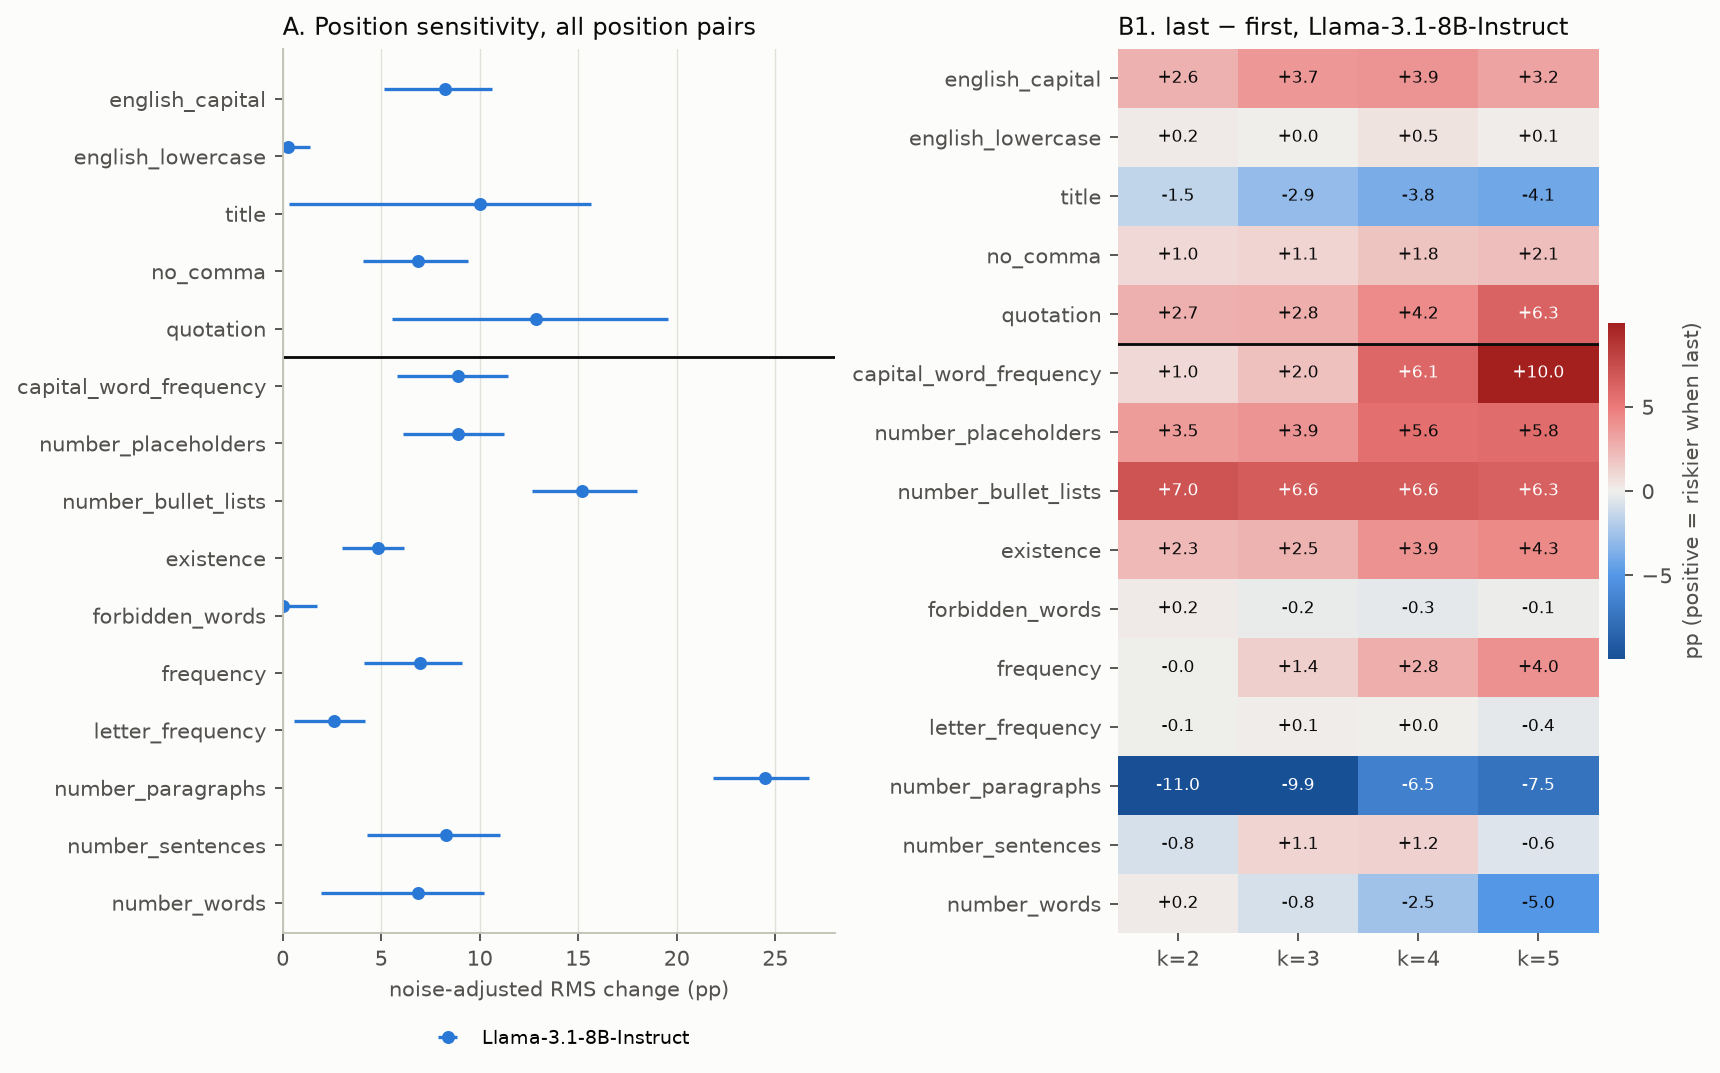
\includegraphics[width=\linewidth]{figures/test_llama/e2_pos_figure.png}
\caption{E2-Pos, Llama, 22 held-out groups (observed). (A) Noise-adjusted RMS change of a rule's violation probability
over all position pairs ($k=2..5$, equal weight per $k$), by target type (fixed-wording types above the line); 95\%
pool-bootstrap intervals. (B) Signed last-minus-first change (points) by type and $k$; positive = riskier when last.
Intervals and support in Appendix Pos-C. Moving a rule also changes its distance to the prompt's end and the placement
of the other rules.}
\label{fig:e2pos}
\end{figure}

\paragraph{Position.} With the exact rule set, task and $k$ fixed, moving a rule changes its violation probability by
a median (over the 15 types) noise-adjusted RMS of 8.2 points (Figure~\ref{fig:e2pos}A), most for paragraph count
(24.5 [21.9, 26.7]) and bullet points (15.2 [12.7, 18.0]), and hardly at all for forbidden words and all-lowercase
(below 0.5). The signed last-minus-first panel (B) is mostly positive: 28 of 60 type--$k$ cells exclude zero, 26 of
them positive (riskier when last), up to $+10.0$ [2.4, 17.6] points for uppercase-word count at $k=5$. Paragraph count
is the exception: it is riskier when first at every $k$ ($-11.0$ [$-18.3$, $-2.2$] at $k=2$).

\begin{figure}[t]
\centering
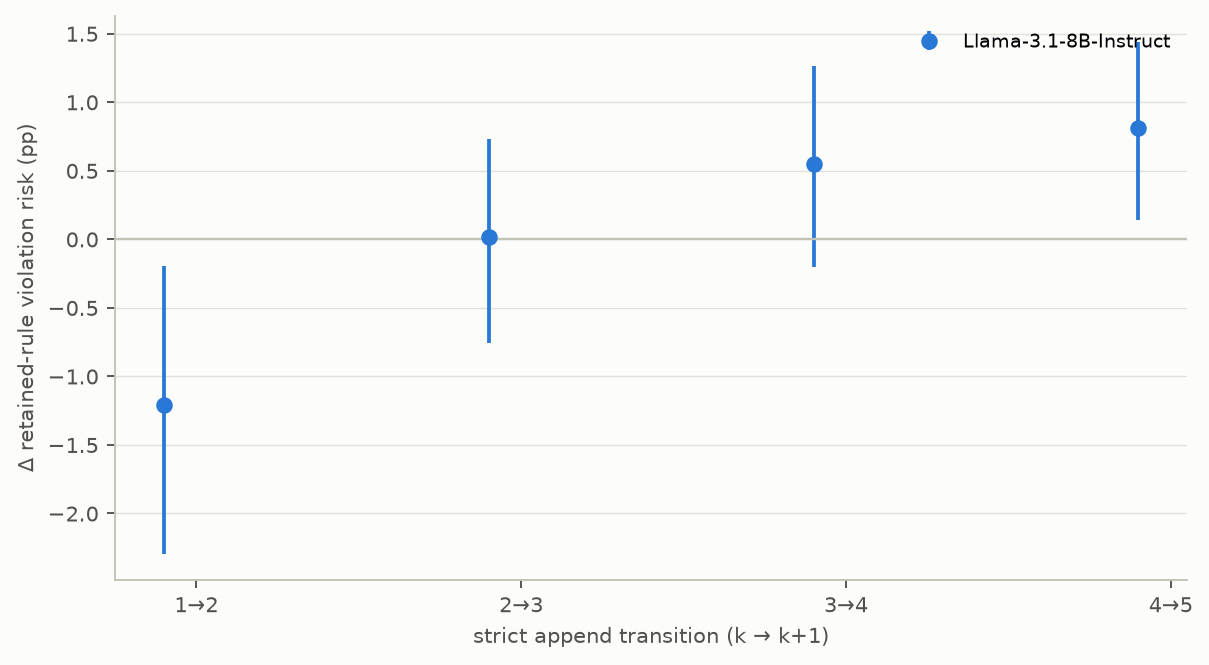
\includegraphics[width=0.72\linewidth]{figures/test_llama/e2_append_figure.png}
\caption{E2-Append, Llama, held-out (observed). Mean change in the violation probability of the retained rules when
one rule is appended to an ordered prefix (the new rule is excluded), by transition; 95\% pool-bootstrap intervals.
$3{\to}4$ and $4{\to}5$ cover only COA orders with an exact prefix.}
\label{fig:e2app}
\end{figure}

\paragraph{Strict append.} Appending one rule moves the risk of the retained rules by about one point
(Figure~\ref{fig:e2app}): $-1.2$ [$-2.3$, $-0.2$] at $1{\to}2$, near zero at $2{\to}3$ and $3{\to}4$, and $+0.8$ [0.1,
1.4] at $4{\to}5$, where the increase falls on the middle slots ($+1.2$ and $+1.3$ for slots 2 and 3) rather than on the
rule that used to be last ($-0.2$; Appendix K-A). A small mean can hide opposing context-specific changes.

\begin{figure}[t]
\centering
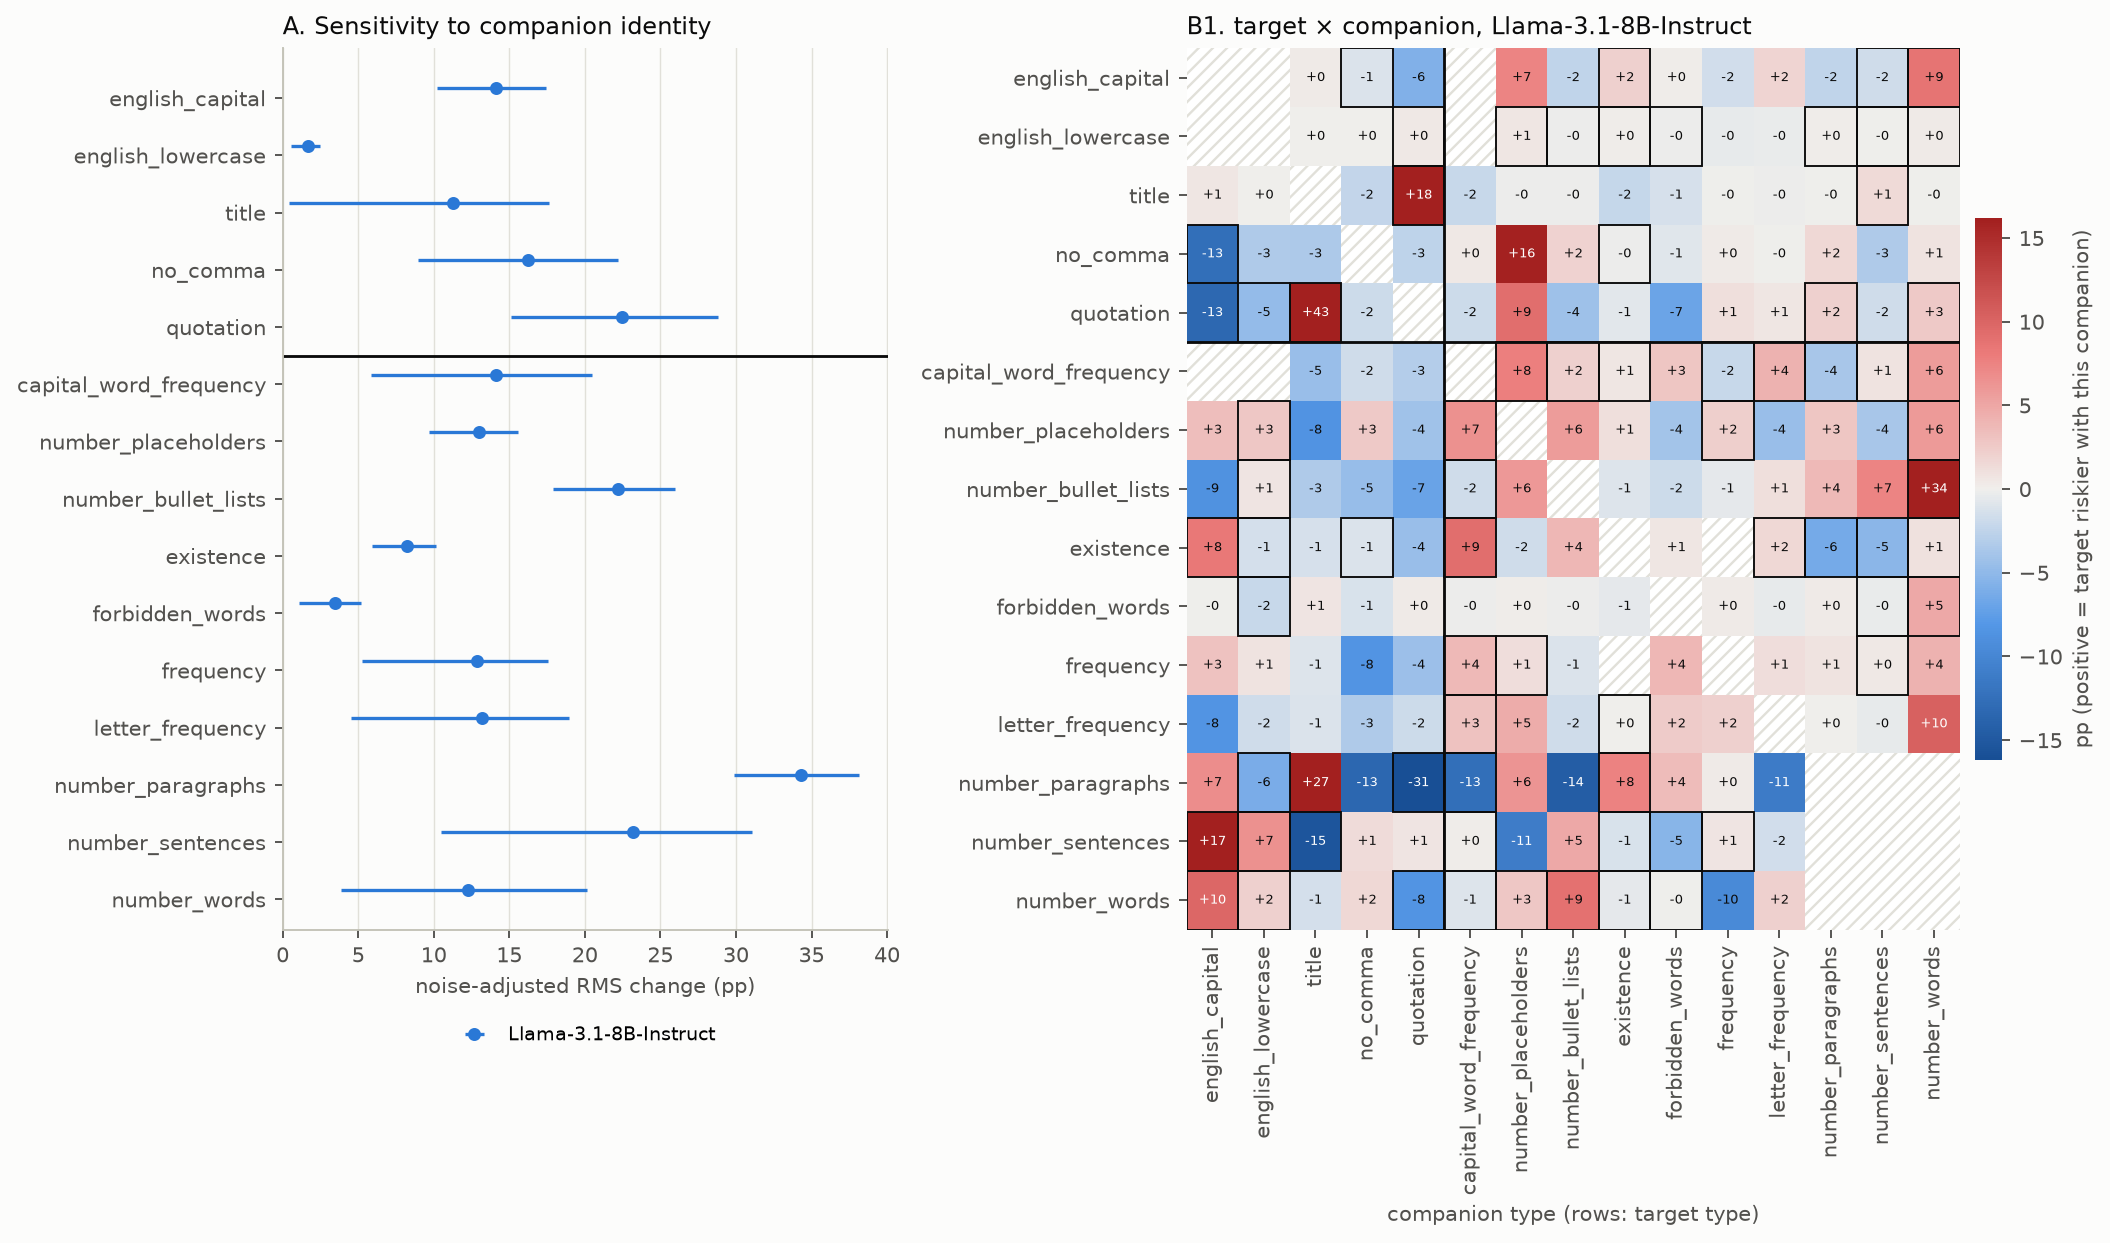
\includegraphics[width=\linewidth]{figures/test_llama/e2_companion_figure.png}
\caption{E2-Companion, Llama, held-out (observed). (A) Noise-adjusted RMS change of the target's violation probability
when exactly one companion (earlier or later) is replaced, by target type ($k=2..5$). (B) Signed target $\times$
companion effects: named companion minus the mean of the other eligible companions in the same fixed context (points);
outlined cells have fewer than 3 pools; hatched cells have no strict match (not zero). Exploratory; numbers in Appendix
C-A.}
\label{fig:e2comp}
\end{figure}

\paragraph{Companion identity.} Replacing a single companion while every other slot stays fixed changes the target's
risk by a median RMS of 13.2 points (Figure~\ref{fig:e2comp}A), most for paragraph count (34.3), sentence count (23.2)
and quotation marks (22.4), and about equally for earlier and later companions (17.2 and 16.5; Appendix C-A).
Companion effects are directed and specific (B): a paragraph-count rule is violated 27.2 [17.5, 37.8] points more often
next to a title rule than next to the alternatives (4 pools), and a no-comma rule 15.9 [9.3, 29.1] points more often
next to a placeholders rule (4 pools). Of the 126 cells with at least 3 pools, 33 have pointwise intervals excluding
zero (about 6 would by chance); they are unadjusted and exploratory.

\begin{figure}[t]
\centering
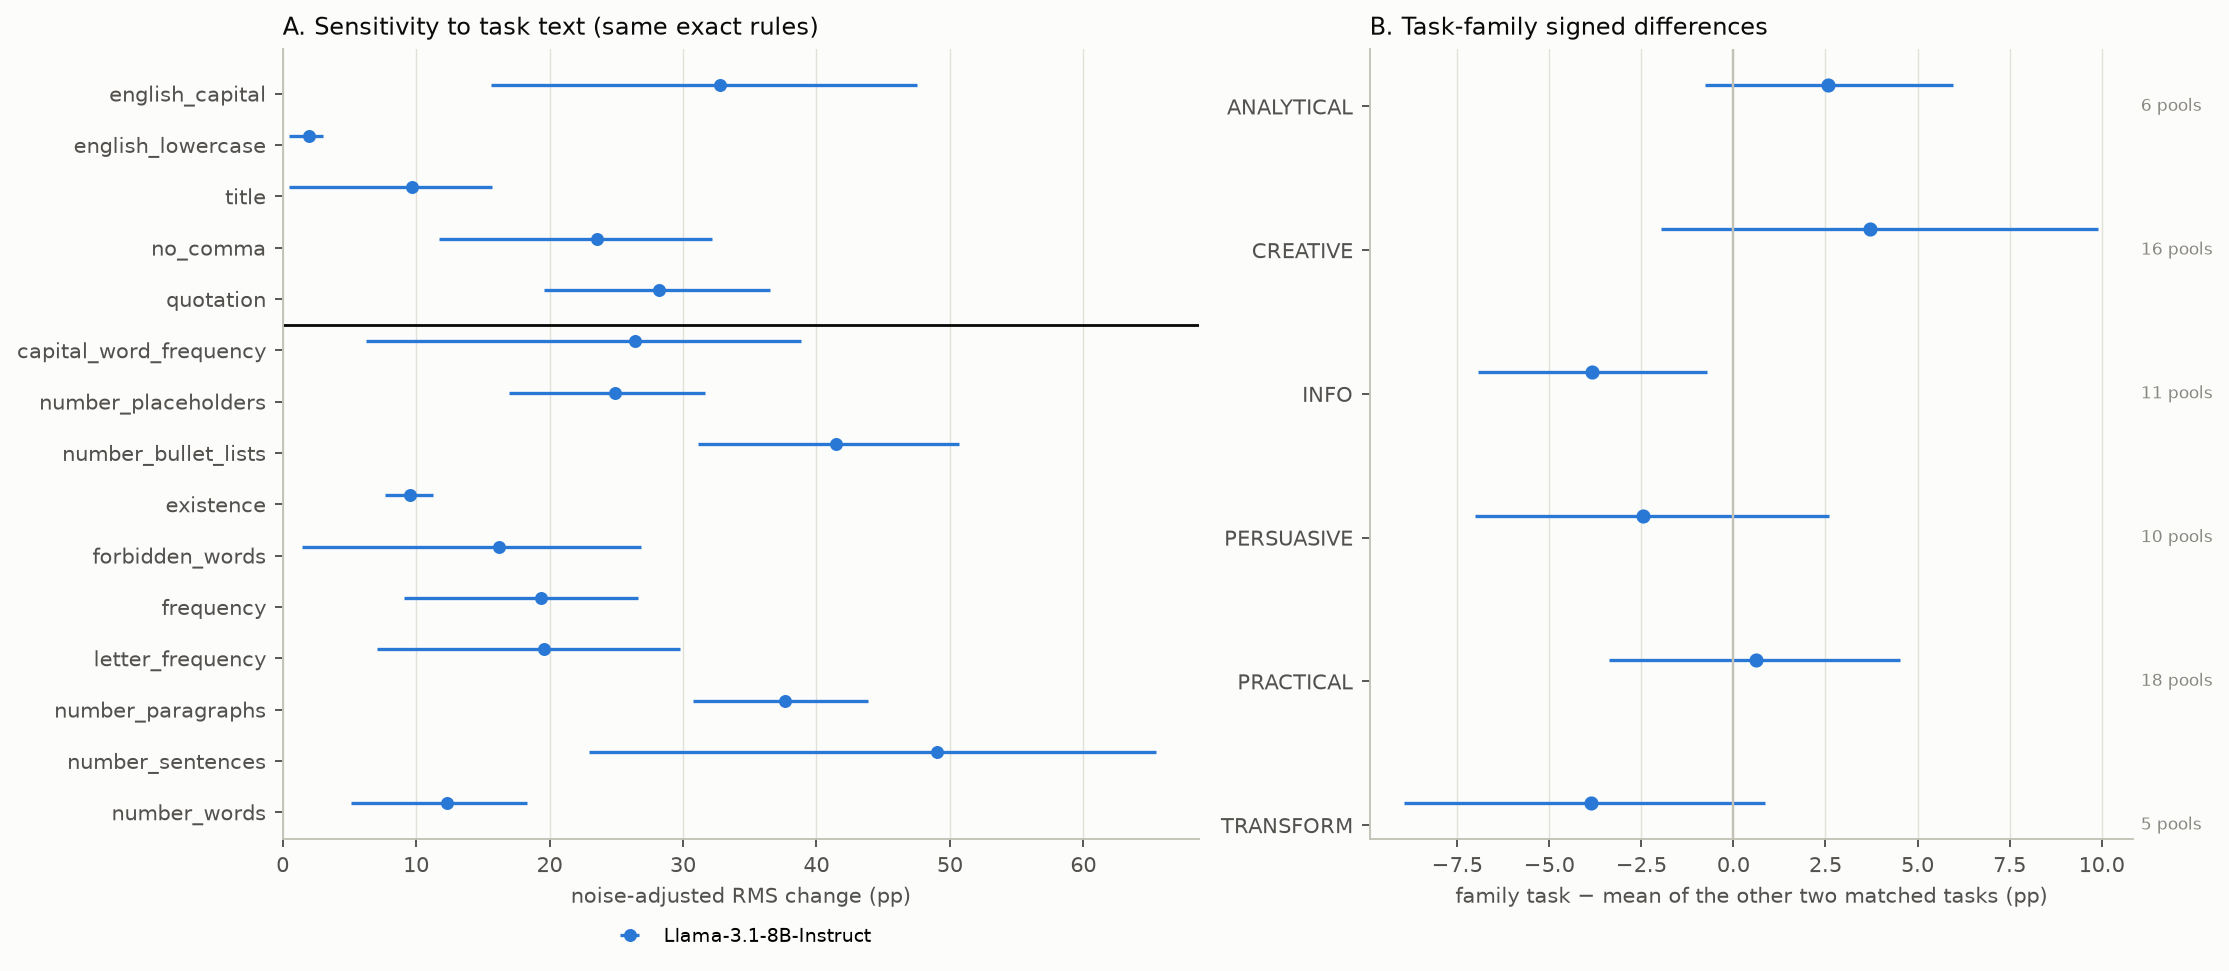
\includegraphics[width=\linewidth]{figures/test_llama/e2_task_figure.png}
\caption{E2-Task, Llama, held-out (observed). (A) Noise-adjusted RMS change when the identical ordered rule
configuration is attached to another task of the same pool, by target type ($k=1..5$). (B) Signed difference between a
family's task and the mean of the other two matched tasks (points), with supporting pools. Families are confounded with
task text; associations, not causal effects.}
\label{fig:e2task}
\end{figure}

\paragraph{Task context.} Changing only the task changes rule risk the most: a median RMS of 23.5 points
(Figure~\ref{fig:e2task}A), up to 49.0 [23.0, 65.4] for sentence count and 41.5 for bullet points, while all-lowercase
stays stable (1.9). By family (B), informational tasks are associated with lower risk than their two matched tasks
($-3.8$ [$-6.9$, $-0.7$] points, 11 pools); no other family's interval excludes zero.

\subsection{Evaluation 2: forecasting the changes}
\label{sec:e2skill}

\begin{table}[t]
\centering\footnotesize
\caption{Evaluation~2, Objective~1 predictor skill on the 22 held-out test groups: paired $\Delta$-MSE reduction ($\times10^{4}$, i.e.\ squared points) [95\% interval] of the predicted versus observed change in a rule's violation probability, MSE(comparator) $-$ MSE(candidate); positive favours the candidate. Position: 57,420 all-pair contrasts; strict append: 69,300 retained-rule contrasts; companion: 177,408 retained-target contrasts; task: 115,236 exact-rule task-pair contrasts (per generator). Equal weight per $k$ (position, companion, task) or transition (append), then pool, task and context. The zero-change row is the MSE of predicting no change. By-stratum values and $\Delta$-MAE in Appendices Pos-B, K-B, C-B and D-C. Qwen: test features still being extracted at the time of this version.}
\label{tab:eval2}
\resizebox{\linewidth}{!}{
\begin{tabular}{llcccc}
\toprule
 & Comparison & Position & Strict append & Companion & Task \\
\midrule
Llama & 1: B1 \cto{} H1 & $-$0.5 [$-$4.6, 3.7] & $-$7.1 [$-$18.6, 3.1] & $-$10.4 [$-$32.9, 11.7] & 94.1 [$-$52.5, 216.8] \\
 & 2: B2 \cto{} H2 & 5.2 [1.9, 8.8] & 1.7 [$-$5.4, 8.5] & 3.7 [$-$10.7, 17.9] & 1.2 [$-$134.6, 119.1] \\
 & 3: B2 \cto{} RCAP & $-$40.3 [$-$58.4, $-$22.6] & $-$22.8 [$-$35.2, $-$9.7] & $-$30.5 [$-$47.6, $-$13.7] & 25.0 [$-$54.2, 111.1] \\
 & 4: H2 \cto{} RCAP & $-$45.6 [$-$65.2, $-$26.8] & $-$24.5 [$-$36.9, $-$11.7] & $-$34.2 [$-$52.2, $-$15.6] & 23.9 [$-$73.9, 139.4] \\
 & 5: B1 \cto{} B1+H1 & $-$1.5 [$-$7.8, 4.9] & $-$5.7 [$-$17.6, 6.6] & $-$6.8 [$-$27.8, 17.1] & $-$7.9 [$-$169.8, 130.9] \\
 & 6: B2 \cto{} B2+H1 & 7.3 [3.9, 11.1] & 6.0 [$-$1.9, 13.6] & 14.1 [1.2, 26.8] & 20.5 [$-$73.4, 110.5] \\
 & 7: B2 \cto{} B2+A1 & $-$18.2 [$-$32.4, $-$4.6] & $-$2.4 [$-$11.9, 7.9] & 0.1 [$-$11.5, 12.5] & 46.3 [$-$19.3, 120.1] \\
 & zero-change MSE & 133.2 & 233.1 & 339.3 & 762.2 \\
\bottomrule
\end{tabular}
}
\end{table}

Table~\ref{tab:eval2} asks whether the predictors forecast these matched changes. The clearest held-out result is
negative for attention: the rule-attention probe forecasts position, append and companion changes worse than B2
(comparison~3: $-40.3$, $-22.8$ and $-30.5$, all intervals below zero), and it also forecasts them worse than H2
(comparison~4, H2 \cto{} RCAP: $-45.6$, $-24.5$ and $-34.2$). The hidden state gives a small, consistent gain for position changes, alone (comparison~2: 5.2 [1.9,
8.8]) and on top of B2 (comparison~6: 7.3 [3.9, 11.1]), where it also improves companion forecasts (14.1 [1.2, 26.8]).
No comparison is clearly better or worse for task changes, which are the noisiest (zero-change MSE 762). Better
absolute accuracy therefore does not imply better forecasts of how a rule's risk moves with its context: rule attention
is the most accurate absolute predictor and the worst forecaster of within-context changes.

% =====================================================================================================
\section{Discussion and limitations}
\label{sec:discussion}

\paragraph{Reading the outcomes.} Comparisons~2 and~3 are the demanding substitutions: B2 already sees the structure,
the prompt and the exact rule, so a candidate that beats it shows that the generator's state exposes information a
frozen encoder of the same prompt does not. On the held-out groups this holds for Llama for both the hidden state and attention (comparisons~2 and~3);
Qwen's test results are pending. The other generator's hidden states matched or beat the generator's own in two of four training-CV cells
(Appendix~\ref{app:cv}), so an internal advantage may reflect a richer encoding of the prompt rather than self-knowledge.
The question is predictive: a win for internal features does not show
that the model ``knows'' it will fail or that attention causes violations \citep{jain2019attention,wiegreffe2019attention};
that needs interventions \citep{li2023iti,stolfo2025steering,zhang2024pasta}.

\paragraph{Limitations.} \emph{Coverage of this version:} test results are for Llama and Objective~1 only; the Objective~2 numbers are grouped-CV estimates on training groups whose folds also selected settings, so they may be optimistic. Evaluation~2 weights follow the plan's proposed recipe, which was not separately signed off before scoring. \emph{Baseline strength:} the text predictors use a frozen encoder; a fine-tuned prompt reader,
as in \citet{ashok2025predict}, could narrow any gap. Only hidden-state predictors get a layer search. \emph{Labels:} each $\phat$ has a standard error up to 0.11, and the ``all uppercase'' verifier can reject correct answers.
\emph{Power and earlier use:} test inference will rest on 22 groups, 16 of which informed earlier design choices
(penalty grids, layer candidates) under a previous split; 46\% of test prompts use subsets outside the training chain
design. \emph{Scope:} two 8B models, English, 15 rule types, at most five compatible rules, single-turn \citep{wallace2024hierarchy,sirdeshmukh2025multichallenge}.


% =====================================================================================================
\section{Conclusion}
\label{sec:conclusion}

On 22 held-out groups of our balanced multi-rule benchmark, Llama~3.1's rule attention and hidden state
forecast per-rule violation risk better than a frozen text predictor that sees the exact rule, yet no predictor
consistently forecasts how that risk changes under controlled edits, and rule attention, the most accurate absolute
predictor, forecasts within-context changes worst. Qwen3 and prompt-level test results will complete the
picture.\label{end:main}

\bibliographystyle{plainnat}
\bibliography{refs}

% =====================================================================================================
\clearpage
\appendix

\section{Study overview}
\label{app:overview}

\begin{figure}[h]
\centering
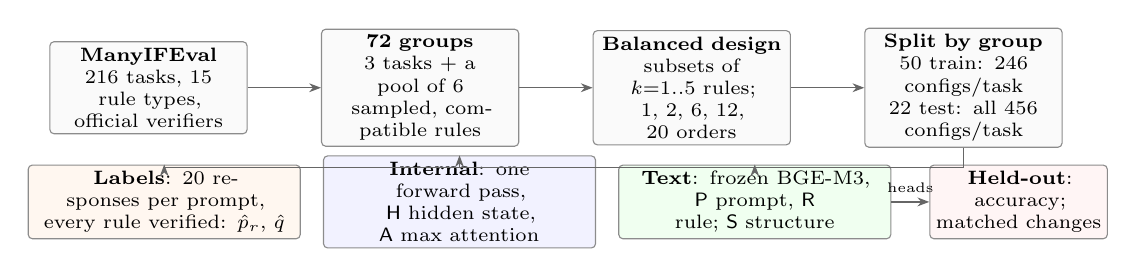
\begin{tikzpicture}[font=\scriptsize,
  box/.style={draw=black!45, rounded corners=1.5pt, align=center, inner sep=2.2pt, text width=#1, fill=black!2},
  box/.default=2.35cm, arr/.style={-{Stealth[length=1.5mm]}, draw=black!60, line width=0.45pt}]
\node[box] (src) at (0,0) {\textbf{ManyIFEval}\\216 tasks, 15 rule types,\\official verifiers};
\node[box] (grp) at (3.45,0) {\textbf{72 groups}\\3 tasks + a pool of 6\\sampled, compatible rules};
\node[box] (des) at (6.9,0) {\textbf{Balanced design}\\subsets of $k{=}1..5$ rules;\\1, 2, 6, 12, 20 orders};
\node[box] (pr) at (10.35,0) {\textbf{Split by group}\\50 train: 246 configs/task\\22 test: all 456 configs/task};
\draw[arr] (src) -- (grp); \draw[arr] (grp) -- (des); \draw[arr] (des) -- (pr);
\node[box=3.3cm, fill=orange!6] (lab) at (0.2,-1.45) {\textbf{Labels}: 20 responses per prompt,\\every rule verified: $\phat_r$, $\qhat$};
\node[box=3.3cm, fill=blue!5] (int) at (3.95,-1.45) {\textbf{Internal}: one forward pass,\\\blk{H} hidden state, \blk{A} max attention};
\node[box=3.3cm, fill=green!6] (txt) at (7.7,-1.45) {\textbf{Text}: frozen BGE-M3,\\\blk{P} prompt, \blk{R} rule; \blk{S} structure};
\node[box=2.1cm, fill=red!4] (ev) at (11.05,-1.45) {\textbf{Held-out}: accuracy;\\matched changes};
\draw[arr] (pr.south) -- ++(0,-0.25) -| (lab.north); \draw[arr] (pr.south) -- ++(0,-0.25) -| (int.north);
\draw[arr] (pr.south) -- ++(0,-0.25) -| (txt.north);
\draw[arr] (txt.east) -- (ev.west) node[midway, above, font=\tiny] {heads};
\end{tikzpicture}
\caption{Overview. Each generator supplies labels (from its sampled responses) and internal feature blocks (from one
forward pass on the prompt alone). Matched heads read different blocks and are compared on held-out groups.}
\label{fig:overview}
\end{figure}

\section{Rule types and an example prompt}
\label{app:types}

\begin{table}[h]
\centering\footnotesize
\caption{The 15 rule types, the parameters drawn by the released code's default generators (``rel.'' is ``less than''
or ``at least'', each with probability one half), and the number of training and test groups whose six-rule pool
contains the type under the adopted split.}
\label{tab:types}
\setlength{\tabcolsep}{3pt}\scriptsize
% generated by report/neurips_draft/make_assets.py -- do not edit
\begin{tabular}{lllcc}
\toprule
Rule type & IFEval identifier & Sampled parameters & Train groups & Test groups \\
\midrule
Include keywords & \texttt{\scriptsize keywords:existence} & 2 keywords & 15 & 7 \\
Keyword count & \texttt{\scriptsize keywords:frequency} & 1 keyword, $N\in[1,3]$, rel. & 18 & 8 \\
Forbidden words & \texttt{\scriptsize keywords:forbidden\_words} & 2 keywords & 29 & 11 \\
Letter count & \texttt{\scriptsize keywords:letter\_frequency} & letter, $N\in[1,10]$, rel. & 29 & 12 \\
Word count & \texttt{\scriptsize length\_constraints:number\_words} & $N\in[100,500]$, rel. & 14 & 6 \\
Sentence count & \texttt{\scriptsize length\_constraints:number\_sentences} & $N\in[1,20]$, rel. & 11 & 7 \\
Paragraph count & \texttt{\scriptsize length\_constraints:number\_paragraphs} & $N\in[1,5]$ & 17 & 8 \\
Placeholders & \texttt{\scriptsize detectable\_content:number\_placeholders} & $N\in[1,4]$ & 27 & 10 \\
Bullet points & \texttt{\scriptsize detectable\_format:number\_bullet\_lists} & $N\in[1,5]$ & 25 & 11 \\
Title & \texttt{\scriptsize detectable\_format:title} & none & 26 & 11 \\
All uppercase & \texttt{\scriptsize change\_case:english\_capital} & none & 18 & 8 \\
All lowercase & \texttt{\scriptsize change\_case:english\_lowercase} & none & 10 & 6 \\
Uppercase-word count & \texttt{\scriptsize change\_case:capital\_word\_frequency} & $N\in[1,20]$, rel. & 12 & 6 \\
Quotation marks & \texttt{\scriptsize startend:quotation} & none & 22 & 10 \\
No commas & \texttt{\scriptsize punctuation:no\_comma} & none & 27 & 11 \\
\bottomrule
\end{tabular}

\end{table}

An example prompt with $k=3$ (rules are rendered verbatim from the released templates):
\begin{quote}\footnotesize\ttfamily
Write a resume for a fresh high school graduate who is seeking their first job.\\[3pt]
Your response should follow the instructions below:\\
- There should be 3 paragraphs. Paragraphs are separated with the markdown divider: ***\\
- Your answer must contain a title, wrapped in double angular brackets, such as <<poem of joy>>.\\
- In your response, the letter i should appear less than 9 times.
\end{quote}

\textbf{Compatibility and feasibility.} Following ManyIFEval, three sets of types are mutually exclusive and never
share a pool: \{keyword existence, keyword frequency\}, the three letter-case types, and \{word, sentence, paragraph
count\}. A parameter draw is rejected only if it is provably unsatisfiable or contradicts another rule in the pool, and
a pool is accepted only when a constructed witness response passes all six official verifiers for each of the group's
three tasks. As in the released prompts, there is no filter on how natural a rule is for a task. The 432 rule instances
are fixed within their group and sampled independently across groups.

\textbf{Generation settings.} We use each model card's default decoding (Llama: temperature 0.6, top-$p$ 0.9; Qwen:
temperature 0.7, top-$p$ 0.8, top-$k$ 20), at most 2,048 new tokens, and vLLM on NVIDIA B200 GPUs. No prompt is
truncated. The verifiers' language detection and sentence splitter are seeded or pinned.

\textbf{Parameter sampling.} We sample parameters only from the released code's default generators and not from the
empirical distribution of the published ManyIFEval prompts. Of the published per-task arguments, 92.3\% are draws from
those defaults, and the remainder were copied from the original hand-written IFEval prompts by an undocumented process;
reproducing that process would require inventing a distribution. Feasibility checks resample only provably
unsatisfiable draws (for example, ``fewer than 1 sentence''), and every rejection is logged with its proof.

\section{Design details}
\label{app:design}

\textbf{Chains.} With the pool in random cyclic order $(\rho_1,\dots,\rho_6)$, chain $c$ is $(\rho_c,\rho_{c+1},\dots,
\rho_{c+4})$ (indices mod 6), and the subset of size $k$ on chain $c$ is its first $k$ rules. Each rule is excluded from
exactly one chain and appears in $k$ of the six subsets of size $k$.

\textbf{COA orders.} Row $\sigma$ of the template for size $k$ is a permutation; the prompt places the subset's
chain-order element $\sigma(p)$ at position $p$. The templates are sharply 2-transitive permutation sets: the identity
for $k=1$, all permutations for $k=2,3$, the 12 even permutations ($A_4$) for $k=4$, and the 20 affine maps
$i\mapsto(ai+b)\bmod 5$, $a\in\{1,\dots,4\}$, $b\in\{0,\dots,4\}$, for $k=5$. For $k\ge2$ each rule appears $k-1$ times
in every position, and every ordered pair of rules appears exactly once at every ordered pair of positions. The design
does not separate higher-order order effects, and for $k\ge4$ it does not cover all $k!$ orders.

\begin{table}[h]
\centering\small
\caption{Counts per task by $k$ in the original design and in the test expansion.}
\label{tab:perk}
\setlength{\tabcolsep}{4pt}\footnotesize
\begin{tabular}{crrrrrr}
\toprule
$k$ & Subsets & Orders/subset & Prompts & Prompt--rule rows & Expanded subsets & Expanded prompts \\
\midrule
1 & 6 & 1 & 6 & 6 & 6 & 6 \\
2 & 6 & 2 & 12 & 24 & 15 & 30 \\
3 & 6 & 6 & 36 & 108 & 20 & 120 \\
4 & 6 & 12 & 72 & 288 & 15 & 180 \\
5 & 6 & 20 & 120 & 600 & 6 & 120 \\
\midrule
Total & 30 & & 246 & 1,026 & 62 & 456 \\
\bottomrule
\end{tabular}
\end{table}

\textbf{Expansion.} For each of the 22 test groups every subset of the six rules at $k=2,3,4$ is included. Existing
subsets keep their original orders exactly (their chain-rotation base order determines which 12 of the 24 orders the
$A_4$ template selects), and new subsets use a fixed base order with the same template. Every original prompt is
reproduced byte for byte under its original identifier, with identical tokenisations for both generators, and the
13,860 new prompts per generator are unique.

\section{Split construction}
\label{app:split}

The split search makes 20,000 seeded random fills of related-task units into 22 test groups and improves each by
best-improvement swaps of equal-sized units, minimising first the shortfall against the hard constraints and then the
balance score (the L1 gap between the test and full-data shares of task families plus that of rule types). Among
admissible results the lowest score wins; 7,916 of the 20,000 draws ended admissible. The adopted split has a balance
score of 0.087, compared with 0.139 for the earlier 15-group split, whose minimum test pair coverage was zero. An exact
solver on pool metadata confirmed that a test coverage of three for every pair is infeasible at any size, because the
pair (uppercase-word count, word count) occurs in only two of the 72 pools; we keep both of its pools in test. The search also requires every type to appear in at least one test and five training groups, keeps clusters of
near-duplicate tasks on one side, and then minimises the family and type imbalance between test and full data. In the
adopted split every pair co-occurs in 2 to 8 test groups, each type appears in 6 to 12 test groups and at least 10
training groups, and 63 of the 98 compatible pairs occur in three or more test groups. Figure~\ref{fig:pairs} shows the full
coverage.

\begin{figure}[h]
\centering
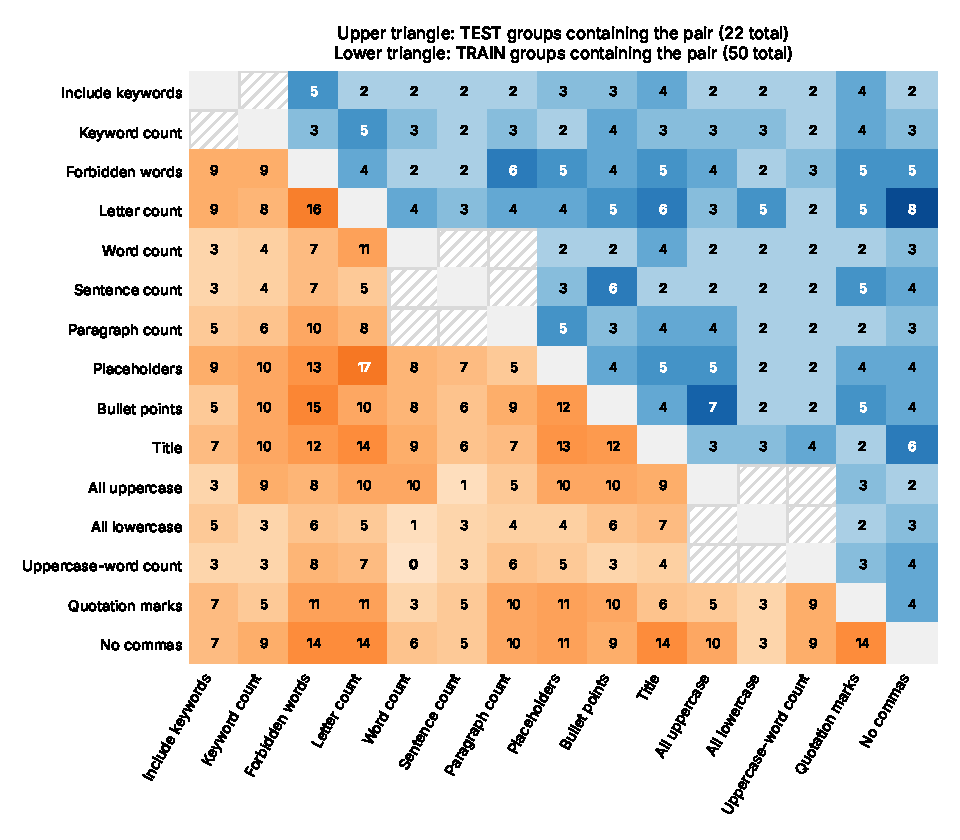
\includegraphics[width=0.8\linewidth]{figures/pair_coverage_s3.pdf}
\caption{Pair coverage of the adopted split: the number of test groups (upper triangle) and training groups (lower
triangle) whose rule pool contains both types. Hatched cells are type pairs that ManyIFEval never combines. Derived
from pool metadata only.}
\label{fig:pairs}
\end{figure}

\section{Feature and fitting details}
\label{app:recipe}

\textbf{Hidden-state rows.} Row 0 holds token embeddings, rows $1,\dots,L-1$ the outputs of decoder layers
$1,\dots,L-1$, row $L$ the last layer after the final normalisation and row $L+1$ the last layer before it ($L=32$ for
Llama, 36 for Qwen). The five candidate depths are 25\%, 37.5\% (38.9\% for Qwen), 50\%, 75\% and 100\%: rows 8, 12, 16, 24 and 33 for Llama and 9, 14, 18, 27 and 37 for Qwen. The
deepest candidate is the un-normalised residual stream of the last layer.

\textbf{Attention extraction.} The eager kernel returns bfloat16 probabilities, so each maximum is itself a bfloat16
value and is stored losslessly. Before the full pass we checked, on fixed training prompts including multi-token rules
and spans whose boundary token straddles whitespace, that each indexed span covers exactly the rule's tokens and that
the extracted value equals the direct maximum from the full attention row for every layer and head.

\textbf{Solver.} Each head is fitted by damped Newton iterations with the exact Hessian (float64 gradient and Cholesky
factorisation), warm-started along the penalty path from strong to weak, and stopped when the largest gradient entry
falls below $10^{-9}$ on the mean scale. Exact-rule embedding blocks are replaced, per head and fold, by coordinates in
an orthonormal basis of their row space on the fitting rows, which is exact for ridge and much faster because a head
sees few distinct rules.

\textbf{Penalty grids.} The structure penalty is $\lambda_S=10$ for Objective~1 and $1$ for Objective~2, on the
summed-loss scale; summing rather than averaging the loss gives every head the same prior strength whatever its size.
$\lambda_X$ and $\lambda_R$ range over $10^2,\dots,10^7$ (Objective~1) and $10^0,\dots,10^5$ (Objective~2). An edge
selection extends that slot's grid by one step, once, for every predictor that uses it. Standardisation uses each
head's fitting rows only. If ``off'' is chosen in an incremental comparison, the gain is zero by construction, which we
do not read as evidence that the block is uninformative.

\textbf{Recipe record.} The fitting recipe (\texttt{configs/v2\_recipe.yaml}) was recorded with SHA-256
\texttt{d286c35b2e0c2c73\ldots} on 2026-11-22 at 23:08 US Eastern time, before any selection reported here. In the
code the addition predictors are named B1+H1, B2+H1 and B2+A1.

\textbf{Ties.} Ties in pooled loss (at a recorded precision) go to the setting with the largest total log-penalty, then
to the larger $\lambda_X$, so selection is deterministic.

\textbf{Sparse heads.} A rule-type head whose fitting rows contain fewer than 50 violated or 50 compliant responses, or
violations in fewer than five groups, is replaced by the intercept-only estimate $(v+0.5)/(n+1)$. The decision depends
only on labels, so such a type contributes identical predictions to both sides of every comparison.

\textbf{Objective~2 weighting.} Each prompt has equal weight in the fractional-logit loss rather than counting its $20k$
checks as separate examples. A sensitivity analysis keeps the per-rule blocks in ordered slots instead of averaging them.

\textbf{Evaluation details.} Probabilities are clipped to $[10^{-6},1-10^{-6}]$ before the logarithm. AUROC is
computed on binary response-level outcomes, not on 20-sample rates, with half credit for ties. Calibration uses ten
bins whose edges are fixed from each predictor's training out-of-fold predictions. The bootstrap uses 10,000 draws of
the 22 test groups, the same draws for every predictor; the sensitivity interval uses a $t_{21}$ reference on
group-level estimates, and leave-one-group-out reruns every headline estimate 22 times.

\textbf{Objective~2 structure.} $k$, rendered prompt length, and for each of five ordered slots the one-hot rule type
(15), span length, distance from the span end to the final token and a presence mask: $2+5\times18=92$ columns.

\section{Evaluation 2: matching, estimands and weights}
\label{app:eval2}

\textbf{Matching.} Every matched pair is built from metadata before outcomes are read, holds the generator, group and
exact rule texts fixed, and is never selected on observed outcomes or on whether a predictor is right. \emph{Position}
holds the task, $k$, the exact subset and the target fixed and compares the target's slots; each slot cell averages the
$k-1$ COA orders that put the target there, with equal weights, so the companions' positions are balanced rather than
fixed. \emph{Strict append} matches an ordered prompt $(r_1,\dots,r_k)$ with $(r_1,\dots,r_k,r_{\text{new}})$ by full
ordered rule identifiers; retained rules are the targets and the new rule is excluded; transitions $3\to4$ and
$4\to5$ cover only the COA orders that contain an exact prefix. \emph{Companion replacement} fixes the task, $k$, the
target and its slot and every other rule and slot, and replaces exactly one companion before or after the target; each
unordered prompt pair is used once per retained target. \emph{Task} keeps the exact configuration and compares the
three tasks of the group pairwise. The counts in Section~\ref{sec:experiments} are design counts; missing or
unverified responses are reported, never filled.

\textbf{Estimands.} Observed effects (Figures~\ref{fig:e2pos}--\ref{fig:e2task}) and predictor skill (Table~\ref{tab:eval2}) are different
quantities. Noise-adjusted RMS sensitivity for a target type averages $d_{\text{obs}}^2-\hat V$ with frozen weights,
where $\hat V$ sums $a_h^2\phat_h(1-\phat_h)/(n_h-1)$ over the prompts $h$ in the two cells with cell weights $a_h$, and
takes $\sqrt{\max(0,\cdot)}$ once; the corrected square is unbiased under independent responses, the clipped root is
not. Signed effects (first-to-last position, appends, a named companion against the equal-weight mean of the eligible
alternatives in the same context, a task family against the other two tasks of its group) are linear and need no
correction. Predictor skill is $\Delta$-MSE; $\Delta$-MAE and a zero-change predictor are reported as checks.
Sign-accuracy on pairs with a reliably non-zero observed change is not used, because filtering on the observed change
selects large, noisy differences.

\textbf{Weights.} Within a pair, retained targets are averaged before pairs are pooled; within a factor, tasks of a
group get equal weight and groups get equal weight; the factor summary averages $k$ values (position, companion, task)
or transitions (append) equally. A micro-weighted score is a sensitivity analysis. Task families are our own labels
and are confounded with task text, and no within-family task comparison exists in this design.

\section{Appendix exhibits: where they are}
\label{app:planned}

The Objective~1 exhibits of the evaluation plan (A1--A4; Pos-A/B/C; K-A/B; C-A/B/C; D-A/B/C/D; Factor E) are
populated from the 22 test groups for Llama in Appendix~\ref{app:test}; Qwen will be added when its test features are
complete. The Objective~2 exhibits (A5--A7 and the Objective~2 matched-change table) remain preliminary training-group
results in Appendix~\ref{app:prelim}.

\section{Held-out test results for Llama: Objective~1 appendix exhibits}
\label{app:test}

\paragraph{Provenance.} Split S3 (\texttt{split-s3-2026-11-23}): the 22 test groups, 66 tasks and all 456 ordered
configurations per task, 30,096 prompts and 115,236 prompt--rule rows, each prompt with 20 verified responses (16,236
original prompts from run \texttt{main}; 13,860 expansion prompts from run \texttt{expansion\_s3\_20261123}, verified
with the same official verifiers). Test hidden states and rule attention were extracted once per prompt with the frozen
backend (HF eager, BF16, Apple MPS) and equal the frozen V1 features bit for bit on the original prompts checked. The
frozen V2 refits on the 50 training groups (\texttt{results/v2\_s3/models/}) were applied once. Code
\texttt{src/mife/eval\_s3/}; tables \texttt{results/eval\_s3/llama\_only/tables/}. Test scoring for Objective~1 was
authorised by the project owner on 24 November 2026; 16 of the 22 test groups were training groups under an earlier
split (Section~\ref{sec:discussion}). Exhibits follow the evaluation plan's Objective~1 appendix layout (A1--A4, Pos,
K, C, D, Factor E).

\subsection*{A1 --- Complete overall metrics (Objective 1)}
\begin{table}[h]
\centering\scriptsize
\caption{A1. Pooled test scores (22 held-out groups; unit: one response $\times$ rule outcome) with 95\% pool-bootstrap intervals. ECE uses ten bins fixed from each predictor's training out-of-fold deciles.}
\label{tab:A1}
\resizebox{\linewidth}{!}{
\begin{tabular}{llcccc}
\toprule
 & Predictor & NLL & Brier & AUROC $\times100$ & ECE $\times100$ \\
\midrule
Llama & Structure only & 0.4077 [0.3636, 0.4534] & 0.1266 [0.1107, 0.1424] & 74.7 [69.5, 79.4] & 5.02 [3.02, 7.26] \\
Llama & B1 & 0.4023 [0.3537, 0.4519] & 0.1245 [0.1072, 0.1416] & 76.6 [72.4, 80.7] & 5.48 [4.06, 7.07] \\
Llama & B2 & 0.3880 [0.3225, 0.4609] & 0.1164 [0.0957, 0.1378] & 81.3 [76.0, 86.1] & 4.30 [2.34, 7.12] \\
Llama & H1+S & 0.3711 [0.3269, 0.4130] & 0.1123 [0.0978, 0.1262] & 81.2 [77.4, 84.7] & 4.17 [2.75, 5.82] \\
Llama & H2+S & 0.3671 [0.3123, 0.4269] & 0.1097 [0.0933, 0.1268] & 83.0 [78.5, 86.9] & 4.20 [2.62, 6.34] \\
Llama & RCAP & 0.3447 [0.2967, 0.3990] & 0.1031 [0.0878, 0.1198] & 83.3 [78.4, 87.5] & 3.17 [1.73, 5.18] \\
Llama & B1+H1 & 0.3892 [0.3406, 0.4340] & 0.1145 [0.0993, 0.1289] & 81.3 [77.6, 84.7] & 5.58 [4.05, 7.27] \\
Llama & B2+H1 & 0.3644 [0.3082, 0.4252] & 0.1083 [0.0911, 0.1260] & 83.2 [78.5, 87.5] & 3.97 [2.33, 6.19] \\
Llama & B2+A1 & 0.3508 [0.2976, 0.4113] & 0.1046 [0.0878, 0.1226] & 83.4 [78.3, 87.8] & 3.49 [2.01, 5.85] \\
\bottomrule
\end{tabular}
}
\end{table}

\begin{table}[h]
\centering\scriptsize
\caption{A1 (contrasts) and A4 (sensitivity). Raw NLL (nats) and AUROC ($\times100$), comparator / candidate; Brier reduction $\times10^3$ with paired interval; NLL-reduction $t_{21}$ jackknife interval and leave-one-pool-out range (nats).}
\label{tab:A1c}
\resizebox{\linewidth}{!}{
\begin{tabular}{llccccc}
\toprule
 & Comparison & NLL comp./cand. & Brier reduction & AUROC comp./cand. & NLL $t_{21}$ interval & NLL leave-one-pool-out \\
\midrule
Llama & 1: B1 \cto{} H1 & 0.4023 / 0.3711 & 12.19 [$-$1.71, 25.54] & 76.6 / 81.2 & [$-$0.0124, 0.0749] & 0.0237 to 0.0433 \\
Llama & 2: B2 \cto{} H2 & 0.3880 / 0.3671 & 6.67 [$-$0.67, 13.91] & 81.3 / 83.0 & [$-$0.0015, 0.0432] & 0.0154 to 0.0275 \\
Llama & 3: B2 \cto{} RCAP & 0.3880 / 0.3447 & 13.25 [4.16, 23.22] & 81.3 / 83.3 & [0.0085, 0.0781] & 0.0333 to 0.0471 \\
Llama & 4: H2 \cto{} RCAP & 0.3671 / 0.3447 & 6.58 [$-$0.65, 14.57] & 83.0 / 83.3 & [$-$0.0078, 0.0526] & 0.0118 to 0.0259 \\
Llama & 5: B1 \cto{} B1+H1 & 0.4023 / 0.3892 & 10.02 [$-$4.18, 23.87] & 76.6 / 81.3 & [$-$0.0346, 0.0608] & 0.0056 to 0.0265 \\
Llama & 6: B2 \cto{} B2+H1 & 0.3880 / 0.3644 & 8.06 [2.33, 14.14] & 81.3 / 83.2 & [0.0052, 0.0419] & 0.0177 to 0.0278 \\
Llama & 7: B2 \cto{} B2+A1 & 0.3880 / 0.3508 & 11.78 [5.53, 18.80] & 81.3 / 83.4 & [0.0141, 0.0603] & 0.0309 to 0.0398 \\
\bottomrule
\end{tabular}
}
\end{table}

\subsection*{A2 --- Calibration (Objective 1)}
\begin{figure}[h]\centering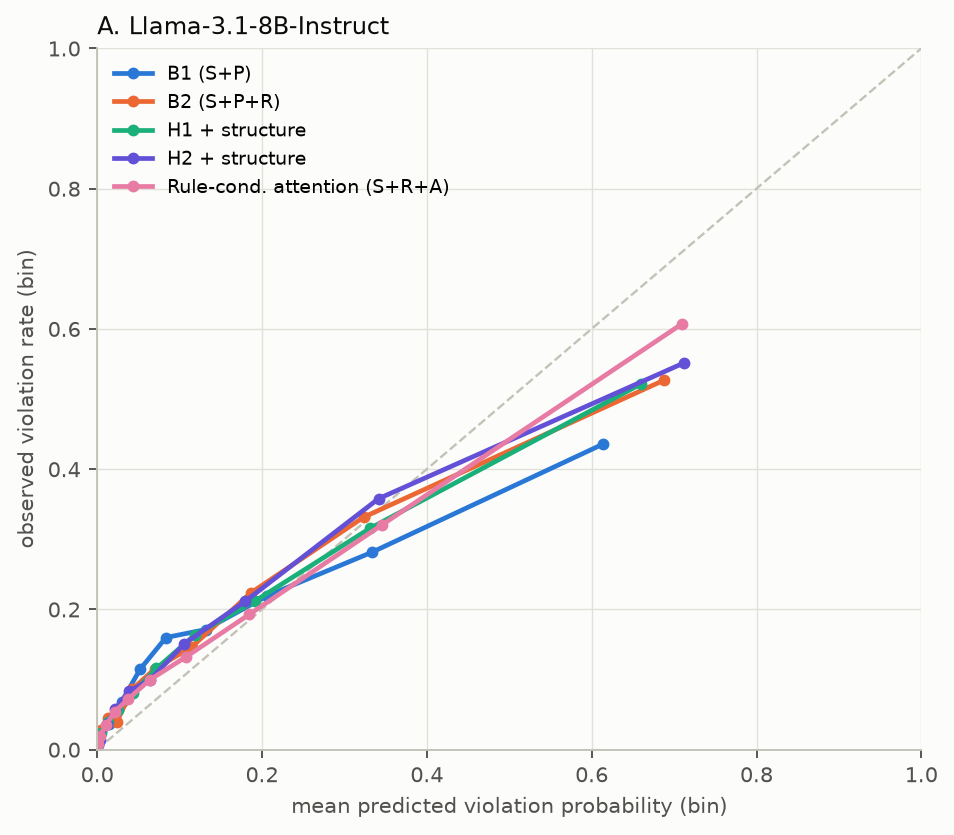
\includegraphics[width=0.62\linewidth]{figures/test_llama/e1_A2_reliability.png}\caption{A2. Reliability curves on the test groups for five key predictors; bins are deciles of each predictor's \emph{training} out-of-fold predictions (fixed before test scoring); unit: response $\times$ rule outcome. Bin support: \texttt{tables/eval1\_calibration.csv}.}\end{figure}
\subsection*{A3 --- Per-type NLL reduction}
\begin{figure}[h]\centering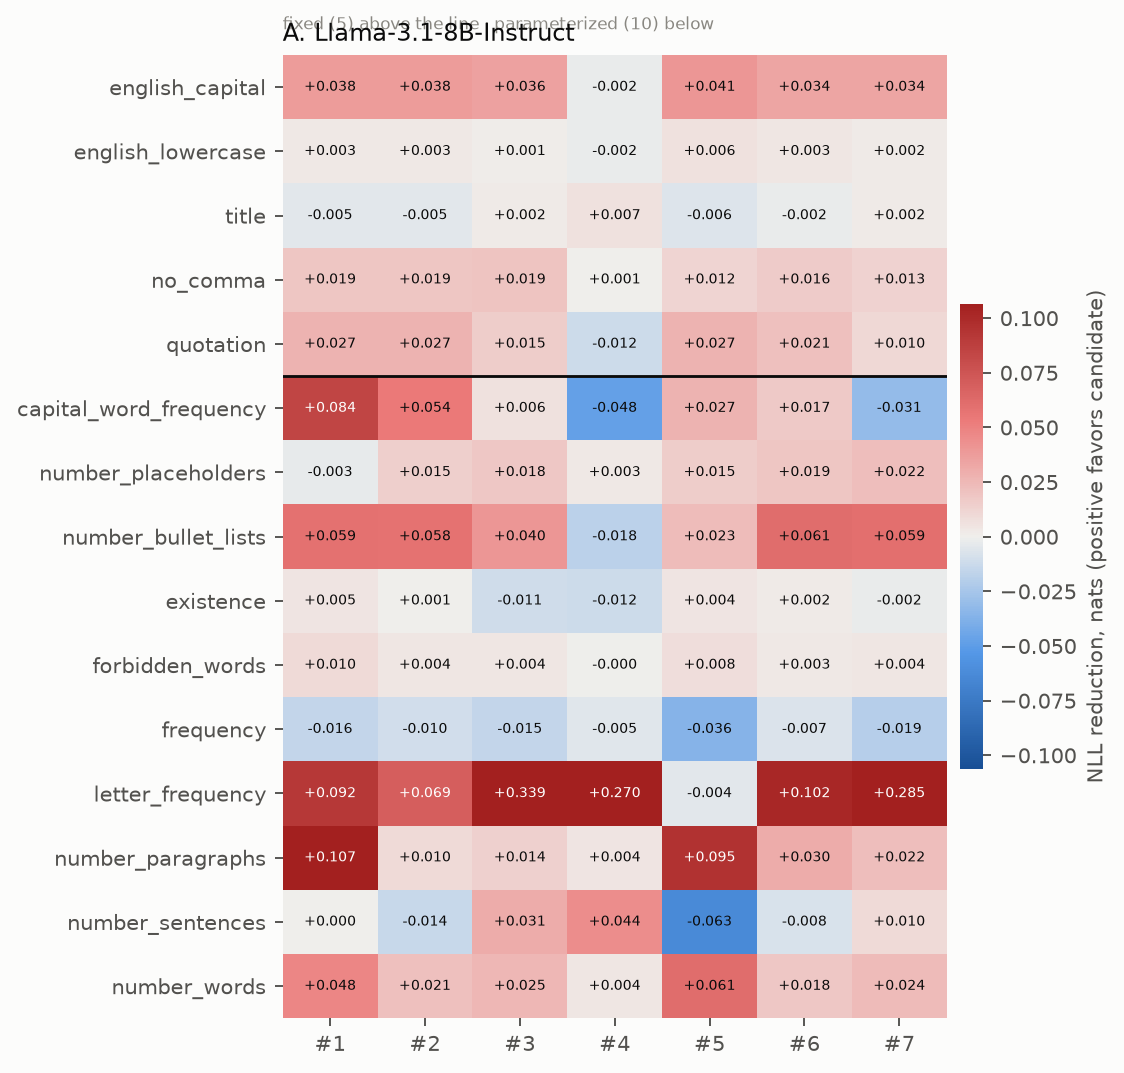
\includegraphics[width=\linewidth]{figures/test_llama/e1_A3_per_type_nll_heatmap.png}\caption{A3. Per-type test NLL reduction (nats) for the seven comparisons; five fixed-wording types above the line, ten parameterised types below; positive (red) favours the candidate. All 210 values per generator with paired intervals and support: \texttt{tables/eval1\_per\_type.csv}.}\end{figure}
\subsection*{A3b --- Fixed versus parameterised rule types (Objective 1 only)}
\begin{table}[h]
\centering\scriptsize
\caption{A3b. NLL reductions of the same seven predictor comparisons, calculated separately on rule-level outcomes from the five fixed and ten parameterised ManyIFEval rule types (nats). Positive improvement favours the candidate (right of the arrow). The fixed-minus-parameterised column compares improvements between subgroups, not raw violation rates. Intervals are paired pointwise 95\% intervals from resampling the 22 test rule pools (identical draws for both classes); all seven subgroup differences are exploratory. Last column: type-equal-weight sensitivity (simple mean of per-type reductions). Observed violation rates: Llama: fixed 8.2\% (803,160 outcomes), parameterised 20.6\% (1,501,560).}
\label{tab:A3b}
\resizebox{\linewidth}{!}{
\begin{tabular}{llcccc}
\toprule
 & Comparison & Fixed $\Delta$NLL & Parameterised $\Delta$NLL & Fixed $-$ param. & Type-equal (F / P) \\
\midrule
Llama & 1: B1 \cto{} H1 & 0.0162 [0.0044, 0.0315] & 0.0393 [$-$0.0240, 0.0996] & $-$0.0232 [$-$0.0850, 0.0403] & 0.0163 / 0.0385 \\
 & 2: B2 \cto{} H2 & 0.0162 [0.0044, 0.0315] & 0.0234 [$-$0.0094, 0.0581] & $-$0.0073 [$-$0.0473, 0.0313] & 0.0163 / 0.0207 \\
 & 3: B2 \cto{} RCAP & 0.0147 [0.0042, 0.0275] & 0.0586 [0.0133, 0.1115] & $-$0.0439 [$-$0.0979, 0.0034] & 0.0146 / 0.0449 \\
 & 4: H2 \cto{} RCAP & $-$0.0015 [$-$0.0073, 0.0048] & 0.0351 [$-$0.0042, 0.0816] & $-$0.0366 [$-$0.0839, 0.0033] & $-$0.0017 / 0.0242 \\
 & 5: B1 \cto{} B1+H1 & 0.0151 [$-$0.0005, 0.0348] & 0.0120 [$-$0.0581, 0.0770] & 0.0031 [$-$0.0647, 0.0753] & 0.0159 / 0.0131 \\
 & 6: B2 \cto{} B2+H1 & 0.0142 [0.0044, 0.0268] & 0.0286 [0.0027, 0.0580] & $-$0.0144 [$-$0.0480, 0.0175] & 0.0144 / 0.0236 \\
 & 7: B2 \cto{} B2+A1 & 0.0120 [0.0040, 0.0216] & 0.0507 [0.0202, 0.0858] & $-$0.0388 [$-$0.0762, $-$0.0055] & 0.0122 / 0.0372 \\
\bottomrule
\end{tabular}
}
\end{table}

\subsection*{A4 --- Technical uncertainty and QC}
Probabilities are clipped to $[10^{-6}, 1-10^{-6}]$ before the logarithm (rows clipped: Llama 28). Every test prompt has 20 distinct verified responses (originals from run \texttt{main}, expansion prompts from run \texttt{expansion\_s3\_20261123}; one decoding-settings hash per generator). The frozen S3 refits were applied once; no sparse-type fallback head fired. New test hidden states and rule-span attention sums equal the frozen V1 features bit for bit on every original prompt checked, and the recomputed BGE-M3 embeddings equal the V1 cache. Bootstrap: 10,000 draws over the 22 test pools, seed 20261203, identical for every predictor, contrast and subgroup; intervals are pointwise and unadjusted. $t_{21}$ jackknife intervals and leave-one-pool-out ranges are in Table~\ref{tab:A1c}. Rule types with fewer than 8 contributing test pools: \texttt{english\_lowercase} (6), \texttt{capital\_word\_frequency} (6), \texttt{existence} (7), \texttt{number\_sentences} (7), \texttt{number\_words} (6). Independent recomputation checks (14/14 passed): direct NLL and \texttt{sklearn} AUROC on expanded binary outcomes; explicit-weight $\Delta$-MSE; structure block reproduces the stored training cache; test and training prompts disjoint.

\subsection*{Pos-A --- Position profiles and all 20 pair strata}
\begin{figure}[h]\centering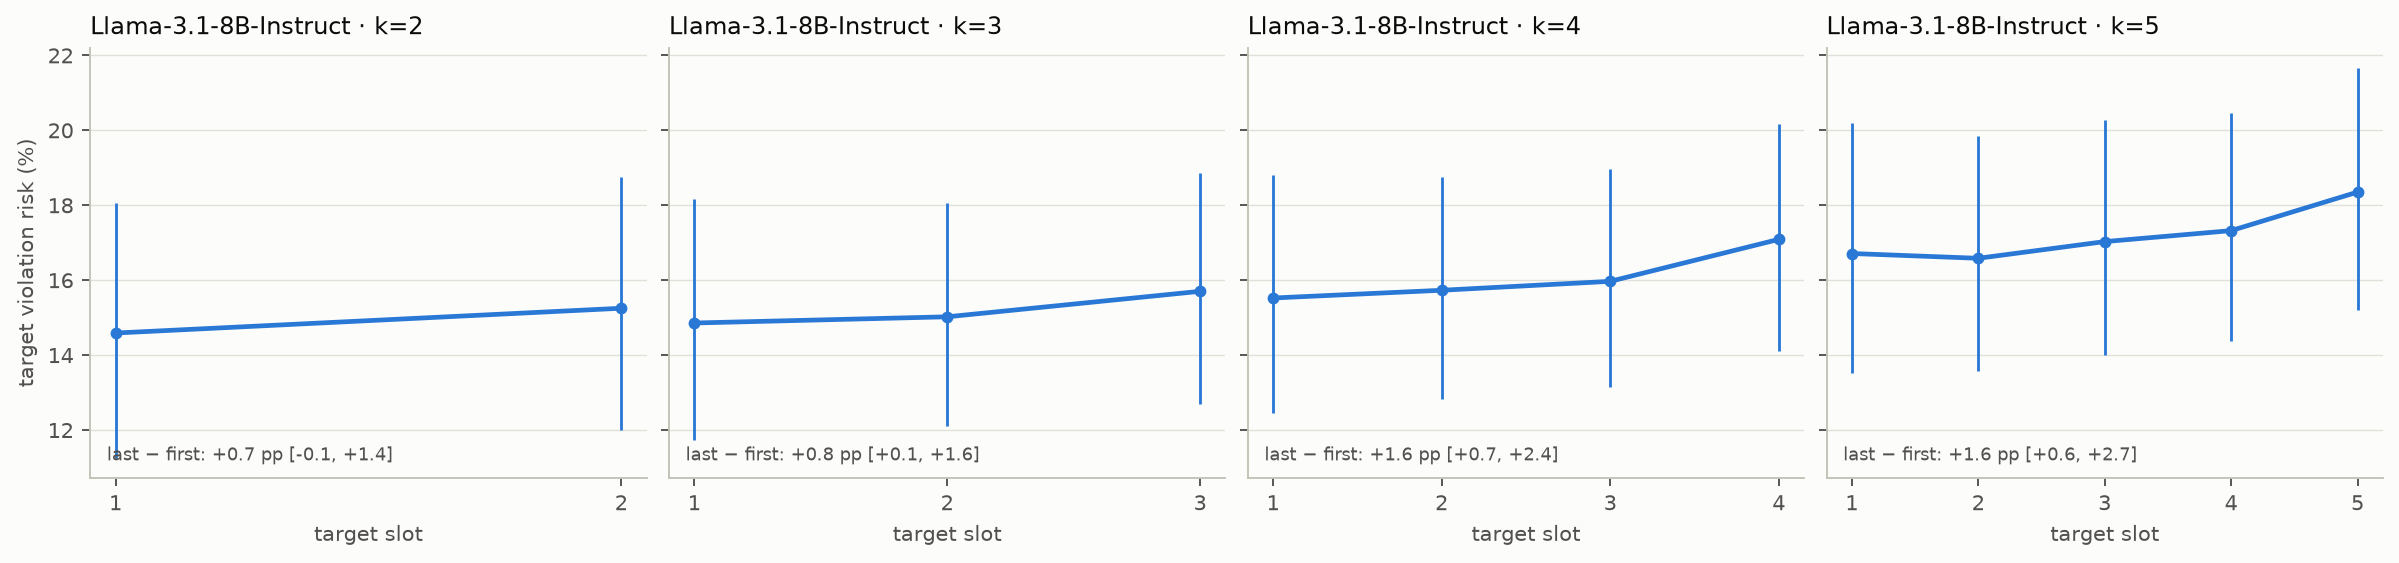
\includegraphics[width=\linewidth]{figures/test_llama/e2_posA_slot_curves.png}\caption{Pos-A. Observed target violation risk at every slot by $k$ (COA-balanced across exact matched contexts, 95\% pool intervals) with the paired last $-$ first difference. Observed outcomes only.}\end{figure}
\begin{table}[h]
\centering\scriptsize
\caption{Pos-A. Signed change (later slot $-$ earlier slot, points) for all 20 position-pair strata, 22 test pools.}
\label{tab:posA}
\begin{tabular}{cccc}
\toprule
$k$ & Slots & Llama & Contexts \\
\midrule
2 & 1$\to$2 & 0.66 [$-$0.13, 1.43] & 1,980 \\
3 & 1$\to$2 & 0.17 [$-$0.40, 0.73] & 3,960 \\
3 & 1$\to$3 & 0.85 [0.07, 1.61] & 3,960 \\
3 & 2$\to$3 & 0.68 [0.33, 1.02] & 3,960 \\
4 & 1$\to$2 & 0.21 [$-$0.41, 0.84] & 3,960 \\
4 & 1$\to$3 & 0.44 [$-$0.34, 1.25] & 3,960 \\
4 & 1$\to$4 & 1.57 [0.70, 2.43] & 3,960 \\
4 & 2$\to$3 & 0.24 [$-$0.03, 0.51] & 3,960 \\
4 & 2$\to$4 & 1.36 [0.77, 1.95] & 3,960 \\
4 & 3$\to$4 & 1.12 [0.52, 1.70] & 3,960 \\
5 & 1$\to$2 & $-$0.13 [$-$0.75, 0.51] & 1,980 \\
5 & 1$\to$3 & 0.32 [$-$0.40, 1.05] & 1,980 \\
5 & 1$\to$4 & 0.61 [$-$0.23, 1.47] & 1,980 \\
5 & 1$\to$5 & 1.64 [0.59, 2.67] & 1,980 \\
5 & 2$\to$3 & 0.45 [0.19, 0.69] & 1,980 \\
5 & 2$\to$4 & 0.74 [0.22, 1.28] & 1,980 \\
5 & 2$\to$5 & 1.77 [0.79, 2.83] & 1,980 \\
5 & 3$\to$4 & 0.29 [$-$0.08, 0.68] & 1,980 \\
5 & 3$\to$5 & 1.32 [0.33, 2.33] & 1,980 \\
5 & 4$\to$5 & 1.03 [0.23, 1.88] & 1,980 \\
\bottomrule
\end{tabular}
\end{table}

\subsection*{Pos-B --- Predicting position changes by $k$}
\begin{table}[h]
\centering\scriptsize
\caption{Pos-B. Paired $\Delta$-MSE reduction ($\times10^4$) [95\% interval] by $k$ on the test groups; positive favours the candidate. Also: zero-change MSE and the $\Delta$-MAE reduction (points) for comparison 2; all $\Delta$-MAE values: \texttt{tables/eval2\_position\_skill.csv}.}
\label{tab:Pos-B}
\resizebox{\linewidth}{!}{
\begin{tabular}{llcccc}
\toprule
 & Comparison & $k$ 2 & $k$ 3 & $k$ 4 & $k$ 5 \\
\midrule
Llama & 1: B1 \cto{} H1 & 1.7 [$-$8.3, 12.0] & 0.9 [$-$4.6, 5.9] & $-$2.6 [$-$5.5, 0.3] & $-$1.8 [$-$5.4, 1.2] \\
 & 2: B2 \cto{} H2 & 11.3 [3.9, 19.7] & 5.4 [1.1, 9.9] & 2.0 [$-$0.8, 5.1] & 2.2 [$-$0.7, 5.4] \\
 & 3: B2 \cto{} RCAP & $-$75.7 [$-$112.2, $-$42.8] & $-$41.1 [$-$61.5, $-$20.0] & $-$28.5 [$-$41.4, $-$14.9] & $-$16.1 [$-$28.0, $-$3.4] \\
 & 4: H2 \cto{} RCAP & $-$87.0 [$-$127.6, $-$50.8] & $-$46.6 [$-$68.2, $-$24.8] & $-$30.5 [$-$43.2, $-$17.5] & $-$18.2 [$-$29.9, $-$6.0] \\
 & 5: B1 \cto{} B1+H1 & $-$4.9 [$-$19.3, 9.3] & $-$2.9 [$-$11.2, 5.3] & $-$1.3 [$-$6.5, 3.9] & 3.0 [$-$3.6, 9.7] \\
 & 6: B2 \cto{} B2+H1 & 15.2 [7.0, 24.7] & 7.4 [3.4, 11.7] & 3.5 [1.3, 5.8] & 3.3 [0.5, 6.3] \\
 & 7: B2 \cto{} B2+A1 & $-$45.0 [$-$77.3, $-$17.1] & $-$19.1 [$-$35.7, $-$2.2] & $-$10.2 [$-$19.5, $-$0.2] & 1.3 [$-$8.4, 12.5] \\
 & zero-change MSE & 186.5 & 127.4 & 111.3 & 107.7 \\
 & $\Delta$-MAE \#2 (pts) & $-$0.10 [$-$0.26, 0.07] & $-$0.02 [$-$0.10, 0.07] & $-$0.01 [$-$0.09, 0.07] & 0.01 [$-$0.07, 0.10] \\
\bottomrule
\end{tabular}
}
\end{table}

\subsection*{Pos-C --- Numerical position estimates and noise diagnostics}
\begin{table}[h]
\centering\scriptsize
\caption{Pos-C (Panel A numbers). Noise-adjusted RMS (points) [95\% interval], corrected squared change and binomial noise floor ($\times10^4$), baseline risk (\%) and pools, by target type.}
\label{tab:posC}
\resizebox{\linewidth}{!}{
\begin{tabular}{lccccc}
\toprule
Type & L RMS & L corr. & L noise & L base & L pools \\
\midrule
\texttt{english\_capital} & 8.2 [5.1, 10.6] & 68.0 & 46.3 & 15.3 & 8 \\
\texttt{english\_lowercase} & 0.3 [0.0, 1.4] & 0.1 & 3.0 & 0.6 & 6 \\
\texttt{title} & 10.0 [0.3, 15.7] & 100.5 & 2.5 & 2.0 & 11 \\
\texttt{no\_comma} & 6.9 [4.1, 9.4] & 47.0 & 19.9 & 7.2 & 11 \\
\texttt{quotation} & 12.9 [5.5, 19.5] & 165.4 & 36.9 & 14.8 & 10 \\
\texttt{capital\_word\_frequency} & 8.9 [5.8, 11.4] & 79.1 & 19.5 & 9.9 & 6 \\
\texttt{number\_placeholders} & 8.9 [6.1, 11.2] & 79.4 & 48.3 & 19.2 & 10 \\
\texttt{number\_bullet\_lists} & 15.2 [12.7, 18.0] & 231.4 & 43.8 & 24.9 & 11 \\
\texttt{existence} & 4.8 [3.0, 6.2] & 23.5 & 28.1 & 8.3 & 7 \\
\texttt{forbidden\_words} & 0.0 [0.0, 1.8] & $-$0.3 & 10.0 & 3.5 & 11 \\
\texttt{frequency} & 7.0 [4.1, 9.1] & 48.4 & 36.1 & 11.8 & 8 \\
\texttt{letter\_frequency} & 2.6 [0.6, 4.2] & 6.7 & 18.0 & 33.6 & 12 \\
\texttt{number\_paragraphs} & 24.5 [21.9, 26.7] & 600.0 & 70.4 & 52.4 & 8 \\
\texttt{number\_sentences} & 8.3 [4.3, 11.0] & 68.4 & 32.3 & 27.2 & 7 \\
\texttt{number\_words} & 6.8 [1.9, 10.2] & 46.9 & 13.0 & 6.5 & 6 \\
\bottomrule
\end{tabular}
}
\end{table}

\begin{table}[h]
\centering\scriptsize
\caption{Pos-C (Panel B numbers). Signed last $-$ first change (points) [pointwise 95\% interval] (supporting pools) by target type and $k$.}
\label{tab:posCs}
\resizebox{\linewidth}{!}{
\begin{tabular}{lcccc}
\toprule
Type & L $k{=}2$ & L $k{=}3$ & L $k{=}4$ & L $k{=}5$ \\
\midrule
\texttt{english\_capital} & 2.6 [$-$0.9, 6.5] (8) & 3.7 [2.0, 5.3] (8) & 3.9 [2.2, 5.9] (8) & 3.2 [1.3, 4.8] (8) \\
\texttt{english\_lowercase} & 0.2 [0.1, 0.3] (6) & 0.0 [$-$0.2, 0.3] (6) & 0.5 [0.2, 0.8] (6) & 0.1 [$-$0.3, 0.6] (6) \\
\texttt{title} & $-$1.5 [$-$3.7, 0.0] (11) & $-$2.9 [$-$7.5, 0.0] (11) & $-$3.8 [$-$9.3, 0.1] (11) & $-$4.1 [$-$10.3, 0.2] (11) \\
\texttt{no\_comma} & 1.0 [$-$0.6, 2.8] (11) & 1.1 [$-$0.4, 2.8] (11) & 1.8 [0.5, 3.2] (11) & 2.1 [0.7, 3.5] (11) \\
\texttt{quotation} & 2.7 [0.5, 5.5] (10) & 2.8 [$-$0.2, 6.6] (10) & 4.2 [1.5, 8.2] (10) & 6.3 [1.2, 13.4] (10) \\
\texttt{capital\_word\_frequency} & 1.0 [$-$1.3, 3.1] (6) & 2.0 [$-$0.9, 4.0] (6) & 6.1 [1.1, 10.9] (6) & 10.0 [2.4, 17.6] (6) \\
\texttt{number\_placeholders} & 3.5 [1.4, 5.6] (10) & 3.9 [0.7, 7.2] (10) & 5.6 [1.0, 10.8] (10) & 5.8 [$-$0.1, 12.1] (10) \\
\texttt{number\_bullet\_lists} & 7.0 [2.8, 11.2] (11) & 6.6 [2.4, 11.1] (11) & 6.6 [2.6, 10.9] (11) & 6.3 [2.1, 10.7] (11) \\
\texttt{existence} & 2.3 [1.3, 3.2] (7) & 2.5 [1.0, 4.1] (7) & 3.9 [2.2, 5.9] (7) & 4.3 [0.9, 7.6] (7) \\
\texttt{forbidden\_words} & 0.2 [$-$0.2, 0.7] (11) & $-$0.2 [$-$0.5, 0.0] (11) & $-$0.3 [$-$0.8, 0.1] (11) & $-$0.1 [$-$0.4, 0.1] (11) \\
\texttt{frequency} & 0.0 [$-$2.9, 2.8] (8) & 1.4 [0.1, 2.6] (8) & 2.8 [0.0, 5.7] (8) & 4.0 [0.7, 8.0] (8) \\
\texttt{letter\_frequency} & $-$0.1 [$-$0.7, 0.8] (12) & 0.1 [$-$1.0, 1.1] (12) & 0.0 [$-$0.8, 0.7] (12) & $-$0.4 [$-$1.4, 0.4] (12) \\
\texttt{number\_paragraphs} & $-$11.0 [$-$18.3, $-$2.2] (8) & $-$9.9 [$-$16.2, $-$1.6] (8) & $-$6.5 [$-$14.1, 0.8] (8) & $-$7.5 [$-$17.4, 3.8] (8) \\
\texttt{number\_sentences} & $-$0.8 [$-$3.7, 0.9] (7) & 1.1 [$-$1.9, 4.0] (7) & 1.2 [$-$1.2, 3.4] (7) & $-$0.6 [$-$2.2, 1.0] (7) \\
\texttt{number\_words} & 0.2 [$-$1.7, 1.8] (6) & $-$0.8 [$-$4.4, 2.5] (6) & $-$2.5 [$-$9.1, 3.0] (6) & $-$5.0 [$-$15.6, 3.3] (6) \\
\bottomrule
\end{tabular}
}
\end{table}

\subsection*{K-A --- Observed append effect by retained slot and transition}
\begin{table}[h]
\centering\scriptsize
\caption{K-A. Mean change in retained-rule violation risk (points) by transition and retained slot $j$ (its absolute position, unchanged by the append); the new rule is excluded; 95\% pool intervals. Coverage: realised strict prefix pairs equal the design (1,980 / 7,920 / 11,880 / 3,960 prompt pairs; 1,980 / 15,840 / 35,640 / 15,840 retained targets); 3$\to$4 and 4$\to$5 cover only COA orders with an exact prefix. Weights: retained targets equal within a pair, then pairs, tasks and pools.}
\label{tab:KA}
\begin{tabular}{cccc}
\toprule
Transition & Slot $j$ & Llama & Pairs / pools \\
\midrule
1$\to$2 & 1 & $-$1.21 [$-$2.30, $-$0.20] & 1,980 / 22 \\
2$\to$3 & 1 & 0.27 [$-$0.54, 1.03] & 7,920 / 22 \\
2$\to$3 & 2 & $-$0.23 [$-$1.06, 0.56] & 7,920 / 22 \\
3$\to$4 & 1 & 0.70 [$-$0.13, 1.51] & 11,880 / 22 \\
3$\to$4 & 2 & 0.66 [$-$0.09, 1.37] & 11,880 / 22 \\
3$\to$4 & 3 & 0.29 [$-$0.54, 1.09] & 11,880 / 22 \\
4$\to$5 & 1 & 0.89 [$-$0.03, 1.80] & 3,960 / 22 \\
4$\to$5 & 2 & 1.21 [0.53, 1.88] & 3,960 / 22 \\
4$\to$5 & 3 & 1.32 [0.65, 2.09] & 3,960 / 22 \\
4$\to$5 & 4 & $-$0.16 [$-$1.09, 0.76] & 3,960 / 22 \\
\bottomrule
\end{tabular}
\end{table}

\subsection*{K-B --- Predicting append changes by transition}
\begin{table}[h]
\centering\scriptsize
\caption{K-B. Paired $\Delta$-MSE reduction ($\times10^4$) [95\% interval] by transition on the test groups; positive favours the candidate. Also: zero-change MSE and the $\Delta$-MAE reduction (points) for comparison 2; all $\Delta$-MAE values: \texttt{tables/eval2\_append\_skill.csv}.}
\label{tab:K-B}
\resizebox{\linewidth}{!}{
\begin{tabular}{llcccc}
\toprule
 & Comparison & transition 1$\to$2 & transition 2$\to$3 & transition 3$\to$4 & transition 4$\to$5 \\
\midrule
Llama & 1: B1 \cto{} H1 & $-$16.1 [$-$40.1, 4.7] & $-$7.6 [$-$19.0, 2.8] & $-$2.3 [$-$10.8, 5.5] & $-$2.3 [$-$10.9, 6.0] \\
 & 2: B2 \cto{} H2 & 0.5 [$-$12.9, 14.2] & 3.9 [$-$4.2, 11.8] & 3.4 [$-$3.6, 10.6] & $-$1.2 [$-$9.4, 6.8] \\
 & 3: B2 \cto{} RCAP & $-$26.9 [$-$52.8, 0.0] & $-$20.4 [$-$34.9, $-$5.2] & $-$17.5 [$-$27.7, $-$7.0] & $-$26.5 [$-$37.4, $-$15.6] \\
 & 4: H2 \cto{} RCAP & $-$27.4 [$-$55.5, 2.2] & $-$24.3 [$-$37.0, $-$11.4] & $-$20.9 [$-$30.7, $-$11.8] & $-$25.4 [$-$38.1, $-$13.2] \\
 & 5: B1 \cto{} B1+H1 & $-$10.8 [$-$33.9, 12.4] & $-$12.9 [$-$27.1, 1.2] & $-$0.7 [$-$11.3, 10.1] & 1.7 [$-$9.5, 13.2] \\
 & 6: B2 \cto{} B2+H1 & 3.1 [$-$11.6, 17.6] & 9.9 [1.2, 18.5] & 8.1 [1.4, 14.9] & 3.1 [$-$3.5, 9.6] \\
 & 7: B2 \cto{} B2+A1 & 0.7 [$-$19.3, 23.2] & $-$0.6 [$-$12.0, 11.2] & $-$0.9 [$-$8.8, 7.4] & $-$8.9 [$-$16.4, $-$0.9] \\
 & zero-change MSE & 276.4 & 229.0 & 219.0 & 208.2 \\
 & $\Delta$-MAE \#2 (pts) & $-$0.20 [$-$0.52, 0.11] & $-$0.05 [$-$0.22, 0.11] & $-$0.02 [$-$0.18, 0.13] & $-$0.09 [$-$0.27, 0.08] \\
\bottomrule
\end{tabular}
}
\end{table}

\subsection*{C-A --- Companion effects: heterogeneity and numerical support}
\begin{table}[h]
\centering\scriptsize
\caption{C-A. Noise-adjusted RMS companion-replacement sensitivity (points) by $k$ and whether the replaced companion is earlier or later than the target (all target types). Signed target $\times$ companion cells (Figure~\ref{fig:e2comp}B) with intervals, pools, tasks, contexts and alternatives: \texttt{tables/eval2\_companion\_signed\_matrix.csv}.}
\label{tab:CA}
\begin{tabular}{cccc}
\toprule
$k$ & Companion & Llama & Comparisons \\
\midrule
2 & earlier & 17.9 [15.6, 19.9] & 3,960 \\
2 & later & 17.4 [15.2, 19.3] & 3,960 \\
2 & both & 17.6 [15.5, 19.4] & 7,920 \\
3 & earlier & 17.2 [15.2, 19.0] & 35,640 \\
3 & later & 16.3 [14.1, 18.3] & 35,640 \\
3 & both & 16.8 [14.7, 18.6] & 71,280 \\
4 & earlier & 16.4 [14.4, 18.2] & 33,264 \\
4 & later & 15.7 [13.5, 17.7] & 33,264 \\
4 & both & 16.0 [14.0, 17.9] & 66,528 \\
5 & earlier & 17.2 [14.8, 19.6] & 15,840 \\
5 & later & 16.4 [13.8, 18.9] & 15,840 \\
5 & both & 16.8 [14.3, 19.2] & 31,680 \\
macro & earlier & 17.2 [15.2, 19.0] & 88,704 \\
macro & later & 16.5 [14.4, 18.4] & 88,704 \\
\bottomrule
\end{tabular}
\end{table}

Llama: 196 of 210 directed off-diagonal cells have strict matches, 70 with fewer than 3 pools; 33 of the 126 cells with at least 3 pools have a pointwise interval excluding zero (about 6 expected by chance if all were null).

\begin{table}[h]
\centering\scriptsize
\caption{C-A (by target type, Panel A numbers). Noise-adjusted RMS (points) [95\% interval], corrected squared change and binomial noise floor ($\times10^4$), baseline risk (\%) and supporting pools.}
\label{tab:CAt}
\resizebox{\linewidth}{!}{
\begin{tabular}{lccccc}
\toprule
Type & L RMS & L corr. & L noise & L base & L pools \\
\midrule
\texttt{english\_capital} & 14.1 [10.2, 17.4] & 200.0 & 84.2 & 15.6 & 8 \\
\texttt{english\_lowercase} & 1.7 [0.6, 2.4] & 2.7 & 5.6 & 0.5 & 6 \\
\texttt{title} & 11.3 [0.4, 17.6] & 127.7 & 6.5 & 2.0 & 11 \\
\texttt{no\_comma} & 16.2 [8.9, 22.2] & 263.2 & 39.9 & 6.6 & 11 \\
\texttt{quotation} & 22.4 [15.1, 28.8] & 503.7 & 72.8 & 14.4 & 10 \\
\texttt{capital\_word\_frequency} & 14.1 [5.9, 20.5] & 198.9 & 42.6 & 9.2 & 6 \\
\texttt{number\_placeholders} & 13.0 [9.7, 15.6] & 168.1 & 99.3 & 17.8 & 10 \\
\texttt{number\_bullet\_lists} & 22.2 [17.9, 26.0] & 491.2 & 85.4 & 25.5 & 11 \\
\texttt{existence} & 8.3 [5.9, 10.2] & 68.1 & 61.5 & 7.7 & 7 \\
\texttt{forbidden\_words} & 3.4 [1.1, 5.2] & 11.8 & 19.6 & 3.1 & 11 \\
\texttt{frequency} & 12.9 [5.2, 17.6] & 166.1 & 70.7 & 11.9 & 8 \\
\texttt{letter\_frequency} & 13.2 [4.5, 18.9] & 173.3 & 33.6 & 32.1 & 12 \\
\texttt{number\_paragraphs} & 34.3 [29.8, 38.2] & 1176.9 & 131.4 & 51.9 & 8 \\
\texttt{number\_sentences} & 23.2 [10.5, 31.1] & 537.6 & 68.9 & 25.4 & 7 \\
\texttt{number\_words} & 12.3 [3.9, 20.2] & 150.1 & 30.4 & 5.7 & 6 \\
\bottomrule
\end{tabular}
}
\end{table}

\subsection*{C-B --- Predicting companion changes by $k$}
\begin{table}[h]
\centering\scriptsize
\caption{C-B. Paired $\Delta$-MSE reduction ($\times10^4$) [95\% interval] by $k$ on the test groups; positive favours the candidate. Also: zero-change MSE and the $\Delta$-MAE reduction (points) for comparison 2; all $\Delta$-MAE values: \texttt{tables/eval2\_companion\_skill.csv}.}
\label{tab:C-B}
\resizebox{\linewidth}{!}{
\begin{tabular}{llcccc}
\toprule
 & Comparison & $k$ 2 & $k$ 3 & $k$ 4 & $k$ 5 \\
\midrule
Llama & 1: B1 \cto{} H1 & $-$3.8 [$-$32.6, 23.8] & $-$11.5 [$-$31.1, 9.0] & $-$17.0 [$-$38.2, 3.8] & $-$9.3 [$-$36.4, 15.9] \\
 & 2: B2 \cto{} H2 & 16.1 [$-$4.3, 37.2] & 5.4 [$-$8.4, 19.3] & $-$1.9 [$-$16.6, 12.0] & $-$4.7 [$-$22.3, 10.9] \\
 & 3: B2 \cto{} RCAP & $-$37.1 [$-$58.7, $-$17.0] & $-$28.6 [$-$45.8, $-$10.7] & $-$31.6 [$-$51.7, $-$11.4] & $-$24.5 [$-$42.7, $-$6.8] \\
 & 4: H2 \cto{} RCAP & $-$53.2 [$-$79.9, $-$27.2] & $-$34.0 [$-$51.4, $-$16.6] & $-$29.7 [$-$49.1, $-$10.0] & $-$19.8 [$-$39.4, 0.4] \\
 & 5: B1 \cto{} B1+H1 & $-$12.2 [$-$43.0, 21.1] & $-$10.5 [$-$31.3, 12.5] & $-$10.8 [$-$30.6, 9.8] & 6.2 [$-$19.0, 32.3] \\
 & 6: B2 \cto{} B2+H1 & 27.3 [7.1, 48.1] & 16.1 [3.2, 28.5] & 8.8 [$-$3.1, 20.3] & 4.1 [$-$9.3, 16.7] \\
 & 7: B2 \cto{} B2+A1 & 4.2 [$-$15.2, 22.9] & 1.1 [$-$12.2, 15.2] & $-$3.7 [$-$16.6, 10.0] & $-$1.3 [$-$14.9, 12.7] \\
 & zero-change MSE & 363.3 & 335.1 & 314.7 & 344.1 \\
 & $\Delta$-MAE \#2 (pts) & 0.09 [$-$0.20, 0.38] & $-$0.02 [$-$0.25, 0.23] & $-$0.05 [$-$0.33, 0.21] & $-$0.07 [$-$0.35, 0.19] \\
\bottomrule
\end{tabular}
}
\end{table}

\subsection*{D-A --- Task sensitivity by target type and $k$}
\begin{table}[h]
\centering\scriptsize
\caption{D-A. Noise-adjusted RMS task sensitivity (points) [95\% interval] by target type and $k$; baseline rates, corrected squares and support in \texttt{tables/eval2\_task\_rms\_type\_k.csv}.}
\label{tab:DA}
\resizebox{\linewidth}{!}{
\begin{tabular}{lccccc}
\toprule
Type & L $k{=}1$ & L $k{=}2$ & L $k{=}3$ & L $k{=}4$ & L $k{=}5$ \\
\midrule
\texttt{english\_capital} & 35.5 [16.9, 51.8] & 32.1 [17.7, 43.3] & 32.8 [15.9, 48.7] & 32.1 [12.7, 50.0] & 31.4 [10.9, 50.2] \\
\texttt{english\_lowercase} & 2.4 [0.0, 4.2] & 2.2 [0.0, 3.5] & 0.9 [0.0, 1.5] & 2.0 [1.2, 2.5] & 1.9 [0.6, 2.6] \\
\texttt{title} & 0.0 [0.0, 0.0] & 9.4 [0.0, 14.9] & 10.2 [0.4, 16.4] & 11.1 [0.6, 17.7] & 12.5 [0.5, 20.7] \\
\texttt{no\_comma} & 30.5 [8.7, 45.5] & 21.9 [9.3, 30.4] & 21.3 [11.7, 29.8] & 21.2 [11.3, 31.3] & 21.3 [10.9, 31.7] \\
\texttt{quotation} & 31.4 [11.5, 45.6] & 27.7 [17.2, 38.9] & 25.9 [18.8, 32.7] & 27.2 [19.1, 34.3] & 28.6 [18.3, 37.2] \\
\texttt{capital\_word\_frequency} & 26.3 [0.0, 45.6] & 26.5 [3.2, 43.5] & 26.7 [5.5, 39.2] & 26.4 [8.4, 39.5] & 26.1 [9.3, 40.7] \\
\texttt{number\_placeholders} & 21.8 [13.5, 28.7] & 24.2 [14.7, 31.5] & 23.9 [16.2, 30.2] & 26.1 [17.8, 32.9] & 28.1 [19.4, 35.5] \\
\texttt{number\_bullet\_lists} & 46.0 [29.4, 59.8] & 42.2 [31.8, 51.2] & 40.1 [30.7, 48.4] & 39.2 [29.3, 48.1] & 39.6 [27.8, 49.4] \\
\texttt{existence} & 6.2 [0.0, 10.3] & 8.7 [6.5, 10.6] & 9.5 [5.8, 12.4] & 10.7 [8.1, 12.9] & 11.6 [7.5, 14.8] \\
\texttt{forbidden\_words} & 15.8 [0.0, 24.0] & 14.9 [0.9, 24.6] & 15.6 [1.0, 26.2] & 16.3 [1.7, 28.1] & 18.3 [2.0, 32.1] \\
\texttt{frequency} & 14.6 [0.0, 25.6] & 18.1 [4.2, 28.1] & 19.9 [7.3, 27.9] & 21.1 [11.2, 28.5] & 22.1 [12.7, 29.1] \\
\texttt{letter\_frequency} & 24.2 [8.8, 37.1] & 23.4 [7.6, 36.0] & 18.7 [5.8, 28.1] & 15.7 [4.2, 23.8] & 13.7 [1.9, 20.8] \\
\texttt{number\_paragraphs} & 41.0 [25.1, 53.7] & 39.0 [27.5, 49.5] & 36.9 [29.2, 43.4] & 35.9 [29.7, 42.7] & 34.9 [28.1, 42.5] \\
\texttt{number\_sentences} & 52.3 [24.6, 69.8] & 49.8 [24.1, 66.4] & 48.8 [20.7, 65.8] & 47.8 [21.8, 64.0] & 46.1 [23.6, 61.8] \\
\texttt{number\_words} & 12.8 [0.0, 22.2] & 11.4 [1.5, 19.1] & 10.4 [3.7, 16.6] & 12.3 [4.7, 19.4] & 14.3 [4.7, 22.3] \\
\bottomrule
\end{tabular}
}
\end{table}

\begin{table}[h]
\centering\scriptsize
\caption{D-A (by target type, Panel A numbers). Noise-adjusted RMS (points) [95\% interval], corrected squared change and noise floor ($\times10^4$), baseline risk (\%) and pools.}
\label{tab:DAt}
\resizebox{\linewidth}{!}{
\begin{tabular}{lccccc}
\toprule
Type & L RMS & L corr. & L noise & L base & L pools \\
\midrule
\texttt{english\_capital} & 32.8 [15.6, 47.5] & 1075.3 & 93.8 & 15.3 & 8 \\
\texttt{english\_lowercase} & 1.9 [0.5, 3.0] & 3.8 & 6.1 & 0.6 & 6 \\
\texttt{title} & 9.7 [0.5, 15.7] & 94.3 & 4.9 & 2.0 & 11 \\
\texttt{no\_comma} & 23.5 [11.7, 32.2] & 554.4 & 41.1 & 7.2 & 11 \\
\texttt{quotation} & 28.2 [19.6, 36.5] & 796.7 & 69.1 & 14.8 & 10 \\
\texttt{capital\_word\_frequency} & 26.4 [6.2, 38.9] & 697.0 & 38.6 & 9.9 & 6 \\
\texttt{number\_placeholders} & 24.9 [17.0, 31.7] & 620.2 & 98.1 & 19.2 & 10 \\
\texttt{number\_bullet\_lists} & 41.5 [31.1, 50.7] & 1722.3 & 79.7 & 24.9 & 11 \\
\texttt{existence} & 9.5 [7.7, 11.3] & 90.6 & 56.0 & 8.3 & 7 \\
\texttt{forbidden\_words} & 16.2 [1.4, 26.9] & 263.4 & 20.1 & 3.5 & 11 \\
\texttt{frequency} & 19.4 [9.1, 26.6] & 374.4 & 66.5 & 11.8 & 8 \\
\texttt{letter\_frequency} & 19.6 [7.1, 29.8] & 383.7 & 36.5 & 33.6 & 12 \\
\texttt{number\_paragraphs} & 37.6 [30.8, 43.8] & 1414.2 & 139.0 & 52.5 & 8 \\
\texttt{number\_sentences} & 49.0 [23.0, 65.4] & 2401.4 & 66.2 & 27.2 & 7 \\
\texttt{number\_words} & 12.3 [5.1, 18.3] & 151.6 & 27.2 & 6.4 & 6 \\
\bottomrule
\end{tabular}
}
\end{table}

\subsection*{D-B --- Rule type $\times$ task family}
\begin{figure}[h]\centering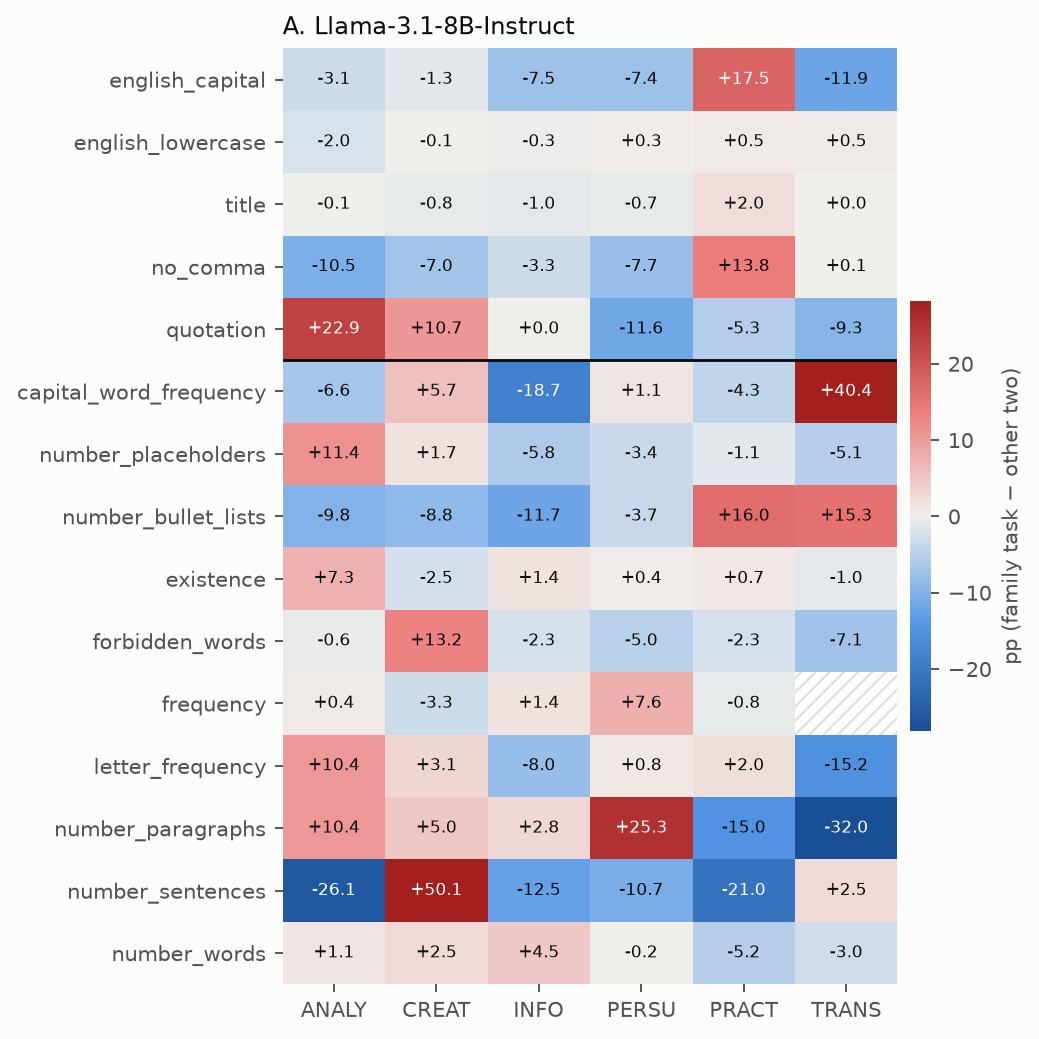
\includegraphics[width=\linewidth]{figures/test_llama/e2_taskDB_type_family_heatmap.png}\caption{D-B. Signed family-task minus mean of the other two matched tasks (points) by target type and family; hatched = unsupported. Descriptive associations; family is confounded with task text. Intervals and support: \texttt{tables/eval2\_task\_type\_family.csv}.}\end{figure}
\begin{table}[h]
\centering\scriptsize
\caption{D-B (family pairs). Within-pool directed family-pair differences (points), shown where at least 3 pools contain both families.}
\label{tab:DBp}
\begin{tabular}{lcc}
\toprule
Family pair & Llama & Pools \\
\midrule
ANALYTICAL $-$ PRACTICAL & $-$1.21 [$-$5.55, 3.60] & 4 \\
CREATIVE $-$ INFO & 6.93 [$-$0.75, 14.97] & 7 \\
CREATIVE $-$ PERSUASIVE & 4.56 [$-$5.58, 15.19] & 7 \\
CREATIVE $-$ PRACTICAL & 2.07 [$-$4.85, 9.56] & 15 \\
INFO $-$ PRACTICAL & $-$1.98 [$-$6.07, 1.64] & 8 \\
INFO $-$ TRANSFORM & 1.28 [$-$8.28, 7.37] & 4 \\
PERSUASIVE $-$ PRACTICAL & $-$3.68 [$-$8.69, 0.52] & 8 \\
\bottomrule
\end{tabular}
\end{table}

\subsection*{D-C --- Predicting task changes by $k$}
\begin{table}[h]
\centering\scriptsize
\caption{D-C. Paired $\Delta$-MSE reduction ($\times10^4$) [95\% interval] by $k$ on the test groups; positive favours the candidate. Also: zero-change MSE and the $\Delta$-MAE reduction (points) for comparison 2; all $\Delta$-MAE values: \texttt{tables/eval2\_task\_skill.csv}.}
\label{tab:D-C}
\resizebox{\linewidth}{!}{
\begin{tabular}{llccccc}
\toprule
 & Comparison & $k$ 1 & $k$ 2 & $k$ 3 & $k$ 4 & $k$ 5 \\
\midrule
Llama & 1: B1 \cto{} H1 & 53.1 [$-$213.8, 278.3] & 96.1 [$-$87.7, 238.7] & 113.8 [$-$20.5, 229.0] & 107.6 [$-$15.7, 218.1] & 100.1 [$-$15.3, 205.8] \\
 & 2: B2 \cto{} H2 & $-$24.5 [$-$274.7, 194.6] & $-$7.5 [$-$172.9, 134.7] & 9.0 [$-$111.9, 119.7] & 14.0 [$-$90.7, 112.5] & 14.8 [$-$77.3, 103.0] \\
 & 3: B2 \cto{} RCAP & $-$28.6 [$-$238.1, 182.2] & 9.4 [$-$110.3, 127.8] & 36.2 [$-$40.1, 115.6] & 49.0 [$-$15.7, 118.3] & 59.3 [$-$0.5, 120.7] \\
 & 4: H2 \cto{} RCAP & $-$4.1 [$-$223.4, 251.8] & 16.9 [$-$114.2, 165.1] & 27.2 [$-$50.2, 117.6] & 34.9 [$-$30.1, 106.8] & 44.5 [$-$12.2, 104.8] \\
 & 5: B1 \cto{} B1+H1 & $-$96.0 [$-$373.8, 151.7] & $-$19.4 [$-$224.9, 143.2] & 25.3 [$-$130.2, 162.0] & 24.3 [$-$124.3, 156.2] & 26.3 [$-$113.4, 149.4] \\
 & 6: B2 \cto{} B2+H1 & $-$19.3 [$-$216.1, 161.0] & 19.6 [$-$98.9, 132.5] & 33.0 [$-$49.9, 116.0] & 34.6 [$-$36.5, 106.6] & 34.5 [$-$26.4, 100.1] \\
 & 7: B2 \cto{} B2+A1 & 38.6 [$-$141.0, 221.2] & 43.4 [$-$40.0, 134.3] & 48.0 [$-$14.1, 113.5] & 48.5 [$-$4.3, 105.5] & 53.3 [9.8, 101.0] \\
 & zero-change MSE & 870.1 & 766.8 & 721.6 & 719.4 & 733.3 \\
 & $\Delta$-MAE \#2 (pts) & 0.19 [$-$1.75, 2.06] & 0.23 [$-$1.14, 1.58] & 0.13 [$-$1.14, 1.37] & 0.12 [$-$1.09, 1.26] & 0.09 [$-$1.03, 1.11] \\
\bottomrule
\end{tabular}
}
\end{table}

\subsection*{C-C and D-D --- Matching, weighting and validation}
Matched pairs are built from manifest metadata only, before outcomes are read, and their counts equal the design counts for every factor and $k$. Companion: same pool, task, $k$, target rule and slot, every other slot identical, exactly one companion differs (earlier and later replacements both included; 7,920 / 35,640 / 22,176 / 7,920 prompt pairs at $k=2..5$). Task: each pool's 456 configurations appear with its three tasks, which belong to three different families, giving three unordered task pairs per target; no within-family matched comparison exists. Weights: equal per $k$ or transition, then pool, task, context and pair (the plan's proposed recipe). The noise-adjusted RMS estimator and its 22-pool interval were checked by simulation before test scoring (\texttt{tables/noise\_validation\_synthetic.csv}, 15 scenarios): the corrected square is unbiased, interval coverage is 91--100\%, and at an exact null the clipped root is biased upward by 0.5--1.1 points, so RMS values below about 1.5 points are not distinguishable from zero. Intervals are pointwise and unadjusted.

\subsection*{Factor E --- Training-defined difficulty terciles}
\begin{table}[h]
\centering\scriptsize
\caption{Factor E. Types grouped by their $k=1$ violation rate on the 50 training groups (5 per tercile, frozen before test scoring); mean test violation rate (\%) and median test noise-adjusted RMS (points) within tercile. Descriptive stratification, not a manipulated factor.}
\label{tab:E}
\begin{tabular}{llccccc}
\toprule
 & Tercile & Train $k{=}1$ rate (\%) & Test rate & Position & Companion & Task \\
\midrule
Llama & easy & 0.0--3.7 & 7.7 & 7.0 & 12.3 & 16.2 \\
 & medium & 5.5--18.1 & 10.1 & 6.9 & 13.0 & 23.5 \\
 & hard & 21.7--47.0 & 29.6 & 8.9 & 22.2 & 37.6 \\
\bottomrule
\end{tabular}
\end{table}


\clearpage
\section{Preliminary training-set results: Objective~2 (provenance and exhibits)}
\label{app:prelim}

\paragraph{Provenance.} Split S3 (\texttt{split-s3-2026-11-23}, applied by \texttt{mife.splits}): 50 training groups,
150 tasks, 36,900 prompts and 153,900 prompt--rule rows per generator, each with 20 verified responses from run
\texttt{main} (3,078,000 rule outcomes per generator). No test-group prompt, label, feature or prediction is read. The
historical 57/15 split and its V1 results are not used. Predictions are the V2 out-of-fold predictions at the
CV-selected setting (\texttt{results/v2\_s3/predictions/}, version \texttt{v2-2026-11-20}, S3 rerun); for every row and
predictor we checked that the stored fold equals the fold of the row's group in \texttt{results/cv\_s3/folds.json}, so
each prediction comes from a model fitted on the other 40 groups. The evaluation code is a copy of the planned test
evaluation re-pointed at the training groups (\texttt{src/mife/prelim\_train/}); outputs are in
\texttt{results/preliminary\_train\_report/}. \emph{Deviations from the plan:} resampling units are 50 training groups,
not 22 test groups; the training design has 246 configurations per task (no strict companion pairs at $k=4$, fewer
append pairs); ECE bins are deciles of the same out-of-fold predictions; Objective~2 uses 2,000 bootstrap draws; the
Objective~2 matched-change analysis (Table~\ref{tab:o2e2}) is a preliminary design choice not fixed by the plan.


Only the Objective~2 exhibits (A5--A7 and the Objective~2 matched-change table) are kept here; the Objective~1 exhibits are replaced by the held-out results in Appendix~\ref{app:test}.

\subsection*{A5 --- Complete overall metrics (Objective 2)}
\begin{table}[h]
\centering\scriptsize
\caption{A5. Out-of-fold prompt-level scores (36,900 prompts). RMSE, MAE and ECE in points; MSE $\times10^4$; correlations $\times100$. Intervals: \texttt{tables/obj2\_eval1\_scores.csv}.}
\label{tab:A5}
\resizebox{\linewidth}{!}{
\begin{tabular}{llcccccc}
\toprule
 & Predictor & RMSE & MAE & MSE & Pearson & Spearman & ECE \\
\midrule
Llama & B1 & 14.62 & 11.59 & 213.6 & 31.4 & 32.9 & 1.94 \\
Llama & B2 & 13.27 & 10.27 & 176.1 & 48.9 & 51.5 & 1.25 \\
Llama & H1+S & 12.67 & 9.40 & 160.6 & 57.5 & 61.5 & 2.50 \\
Llama & H2+S & 12.67 & 9.64 & 160.5 & 55.7 & 60.0 & 1.69 \\
Llama & RCAP & 12.51 & 9.50 & 156.6 & 57.5 & 59.9 & 1.65 \\
Llama & B1+H1 & 12.69 & 9.42 & 161.2 & 57.3 & 61.3 & 2.51 \\
Llama & B2+H1 & 12.73 & 9.61 & 162.0 & 55.3 & 59.9 & 1.77 \\
Llama & B2+A1 & 12.52 & 9.51 & 156.7 & 57.4 & 59.7 & 1.62 \\
Llama & Structure only & 14.77 & 11.78 & 218.3 & 28.8 & 29.9 & 2.21 \\
\midrule
Qwen & B1 & 11.80 & 8.73 & 139.3 & 30.2 & 35.0 & 1.70 \\
Qwen & B2 & 11.50 & 8.41 & 132.2 & 36.0 & 36.0 & 1.57 \\
Qwen & H1+S & 11.04 & 7.78 & 121.9 & 46.1 & 47.1 & 1.82 \\
Qwen & H2+S & 11.01 & 7.76 & 121.2 & 46.4 & 47.3 & 1.83 \\
Qwen & RCAP & 11.00 & 7.91 & 121.1 & 44.7 & 46.5 & 1.56 \\
Qwen & B1+H1 & 11.06 & 7.79 & 122.2 & 45.8 & 47.0 & 1.83 \\
Qwen & B2+H1 & 11.04 & 7.77 & 121.9 & 45.9 & 47.4 & 1.99 \\
Qwen & B2+A1 & 11.19 & 7.98 & 125.1 & 42.3 & 45.0 & 1.78 \\
Qwen & Structure only & 11.84 & 8.79 & 140.2 & 29.8 & 34.4 & 1.78 \\
\bottomrule
\end{tabular}
}
\end{table}

\begin{table}[h]
\centering\scriptsize
\caption{A5 (contrasts). MAE reduction (points), MSE reduction ($\times10^4$) and Pearson gain ($\times100$).}
\label{tab:A5c}
\resizebox{\linewidth}{!}{
\begin{tabular}{llccc}
\toprule
 & Comparison & MAE reduction & MSE reduction & Pearson gain \\
\midrule
Llama & 1: B1 \cto{} H1 & 2.19 [1.19, 3.25] & 53.1 [22.2, 84.4] & 26.1 [15.6, 37.8] \\
Llama & 2: B2 \cto{} H2 & 0.63 [0.12, 1.18] & 15.6 [0.9, 30.7] & 6.8 [2.0, 12.9] \\
Llama & 3: B2 \cto{} RCAP & 0.77 [0.23, 1.36] & 19.5 [1.5, 37.8] & 8.6 [2.3, 15.1] \\
Llama & 4: H2 \cto{} RCAP & 0.14 [$-$0.28, 0.56] & 3.9 [$-$11.4, 18.1] & 1.8 [$-$3.7, 6.5] \\
Llama & 5: B1 \cto{} B1+H1 & 2.18 [1.17, 3.24] & 52.5 [21.7, 83.9] & 25.9 [15.3, 37.7] \\
Llama & 6: B2 \cto{} B2+H1 & 0.66 [0.18, 1.21] & 14.0 [$-$0.7, 29.5] & 6.5 [1.7, 12.6] \\
Llama & 7: B2 \cto{} B2+A1 & 0.76 [0.23, 1.35] & 19.3 [1.8, 37.5] & 8.5 [2.1, 15.1] \\
\midrule
Qwen & 1: B1 \cto{} H1 & 0.95 [0.33, 1.58] & 17.4 [$-$2.5, 36.9] & 16.0 [5.6, 26.7] \\
Qwen & 2: B2 \cto{} H2 & 0.66 [0.03, 1.27] & 11.0 [$-$10.1, 31.0] & 10.4 [$-$1.3, 22.7] \\
Qwen & 3: B2 \cto{} RCAP & 0.50 [0.10, 0.91] & 11.2 [$-$1.0, 23.8] & 8.8 [0.8, 17.6] \\
Qwen & 4: H2 \cto{} RCAP & $-$0.15 [$-$0.54, 0.28] & 0.2 [$-$13.0, 15.9] & $-$1.7 [$-$8.6, 5.6] \\
Qwen & 5: B1 \cto{} B1+H1 & 0.94 [0.33, 1.56] & 17.1 [$-$2.6, 36.1] & 15.7 [5.3, 26.4] \\
Qwen & 6: B2 \cto{} B2+H1 & 0.65 [0.09, 1.20] & 10.4 [$-$6.6, 26.8] & 9.9 [0.5, 20.4] \\
Qwen & 7: B2 \cto{} B2+A1 & 0.43 [0.12, 0.74] & 7.1 [$-$1.5, 15.7] & 6.3 [0.9, 12.7] \\
\bottomrule
\end{tabular}
}
\end{table}

\subsection*{A6 --- Fraction calibration (Objective 2)}
\begin{table}[h]
\centering\scriptsize
\caption{A6. Mean predicted / mean observed fraction violated (points) in decile bins of each predictor's out-of-fold predictions ($\approx$3,690 prompts per bin). All predictors: \texttt{tables/obj2\_eval1\_calibration.csv}.}
\label{tab:A6}
\begin{tabular}{llp{0.62\linewidth}}
\toprule
 & Predictor & Bins 1--10: predicted/observed \\
\midrule
Llama & B2 & 6/6, 9/8, 11/10, 12/13, 14/14, 16/18, 18/21, 21/22, 24/25, 34/31 \\
Llama & H2+S & 5/5, 7/7, 9/8, 11/12, 13/14, 15/17, 18/21, 21/23, 25/27, 36/33 \\
Llama & RCAP & 4/5, 7/7, 9/9, 11/11, 13/14, 15/18, 17/20, 20/22, 25/26, 38/34 \\
Qwen & B2 & 2/3, 3/4, 4/6, 5/8, 6/9, 8/9, 9/9, 11/11, 15/15, 22/17 \\
Qwen & H2+S & 1/2, 2/3, 3/5, 4/6, 5/7, 6/9, 8/10, 10/12, 14/14, 26/22 \\
Qwen & RCAP & 1/2, 3/3, 4/5, 5/6, 6/8, 7/9, 9/11, 11/12, 14/14, 24/20 \\
\bottomrule
\end{tabular}
\end{table}

\subsection*{A7 --- Reference predictions (Objective 2)}
\begin{table}[h]
\centering\scriptsize
\caption{A7. Training-fold mean and averaged Objective~1 predictions as references (not among the seven comparisons).}
\label{tab:A7}
\begin{tabular}{llcc}
\toprule
 & Reference & RMSE (pp) & Spearman $\times100$ \\
\midrule
Llama & Training-fold mean & 15.34 & undefined (constant per fold) \\
Llama & Mean of Obj.~1 B2 & 13.02 & 58.5 \\
Llama & Mean of Obj.~1 H2 & 12.22 & 62.7 \\
Llama & Mean of Obj.~1 RCAP & 12.50 & 61.5 \\
Llama & Obj.~2 head H2+S & 12.67 & 60.0 \\
\midrule
Qwen & Training-fold mean & 12.31 & undefined (constant per fold) \\
Qwen & Mean of Obj.~1 B2 & 11.17 & 42.8 \\
Qwen & Mean of Obj.~1 H2 & 11.02 & 48.1 \\
Qwen & Mean of Obj.~1 RCAP & 10.86 & 49.7 \\
Qwen & Obj.~2 head H2+S & 11.01 & 47.3 \\
\bottomrule
\end{tabular}
\end{table}

\subsection*{Evaluation 2, Objective 2 (preliminary design, not fixed by the plan)}
\begin{table}[h]
\centering\scriptsize
\caption{Objective~2 matched changes: prompt-level pairs, outcome = fraction of rules violated. Observed noise-adjusted RMS and signed mean (points; append includes the new rule, so the denominator changes); zero-change MSE and $\Delta$-MSE ($\times10^4$) for the primary comparisons. Secondary comparisons: \texttt{tables/obj2\_eval2.csv}.}
\label{tab:o2e2}
\resizebox{\linewidth}{!}{
\begin{tabular}{llcccccccc}
\toprule
 & Factor & Pairs & RMS & Signed mean & Zero MSE & 1 & 2 & 3 & 4 \\
\midrule
Llama & position & 244,800 & 6.9 [6.0, 7.7] & $-$0.08 [$-$0.35, 0.22] & 65.4 & $-$6.2 [$-$9.9, $-$2.3] & $-$3.7 [$-$5.9, $-$1.6] & $-$15.3 [$-$22.3, $-$8.9] & $-$11.6 [$-$17.3, $-$6.4] \\
 & append & 14,400 & 15.4 [14.1, 16.6] & 0.49 [$-$0.02, 1.01] & 259.8 & 57.8 [39.9, 76.4] & 16.1 [6.2, 26.8] & 14.4 [0.3, 28.8] & $-$1.7 [$-$15.3, 10.7] \\
 & companion & 25,200 & 16.7 [15.3, 18.1] & $-$0.22 [$-$1.12, 0.74] & 299.5 & 54.2 [29.6, 79.9] & 26.0 [14.4, 39.0] & 15.0 [$-$0.8, 32.7] & $-$11.0 [$-$24.7, 2.1] \\
 & task & 36,900 & 18.8 [16.9, 20.5] & $-$0.42 [$-$2.12, 1.22] & 376.3 & $-$3.1 [$-$42.1, 37.9] & 9.2 [$-$14.7, 34.1] & 13.5 [$-$28.3, 56.1] & 4.3 [$-$29.1, 35.0] \\
\midrule
Qwen & position & 244,800 & 6.1 [5.4, 6.8] & 0.06 [$-$0.07, 0.20] & 45.1 & $-$5.6 [$-$8.9, $-$2.8] & $-$5.6 [$-$8.7, $-$2.8] & $-$6.2 [$-$9.3, $-$3.6] & $-$0.6 [$-$2.6, 1.3] \\
 & append & 14,400 & 12.0 [10.5, 13.4] & 1.09 [0.72, 1.48] & 152.2 & 17.0 [8.6, 26.5] & 7.0 [$-$3.3, 17.2] & 9.8 [$-$0.4, 21.8] & 2.8 [$-$5.4, 11.1] \\
 & companion & 25,200 & 13.4 [11.7, 15.0] & 0.28 [$-$0.53, 1.17] & 188.0 & 20.7 [10.7, 32.2] & 12.7 [0.7, 25.6] & 6.5 [$-$4.3, 18.3] & $-$6.3 [$-$15.2, 1.9] \\
 & task & 36,900 & 12.6 [10.8, 14.2] & $-$0.44 [$-$1.67, 0.72] & 166.9 & $-$12.2 [$-$29.1, 2.9] & $-$11.8 [$-$28.9, 3.7] & $-$4.3 [$-$19.9, 12.2] & 7.5 [$-$3.8, 20.5] \\
\bottomrule
\end{tabular}
}
\end{table}


\clearpage
\section{Training cross-validation diagnostics}
\label{app:cv}

Table~\ref{tab:cv} lists the pooled cross-validation loss of each predictor at its selected setting. These are the
criteria used for selection, computed on the 50 training groups only; they are optimistically biased, carry no
uncertainty estimate and are \emph{not} estimates of held-out performance. They are reported to document the selection,
not to support any comparison. Two features matter for reading the test results. First, the frozen prompt embedding
adds little to structure alone (B1 vs structure only), so B2's advantage over B1 comes mostly from the exact-rule
embedding. Second, the other generator's hidden states (last row; its layer was selected the same way) score better
than the generator's own H1 for Llama in Objective~1 and for Qwen in Objective~2, and worse in the other two cells. Third, for Objective~2 the mean of the Objective~1 out-of-fold predictions over a
prompt's rules is often more accurate than the dedicated prompt-level heads (for Llama, the averaged H2 predictions
reach $14.9\times10^{-3}$ against $15.7\times10^{-3}$ for the best dedicated head), so the averaged reference is a strong
comparator for Table~\ref{tab:e1o1}.

\begin{table}[h]
\centering\footnotesize
\caption{Training cross-validation loss at the selected setting (5 grouped folds over the 50 training groups) and the
number of input features. Objective~1: pooled mean log loss per completion. Objective~2: pooled squared error of
$\hat q$, $\times10^3$. Generated from \texttt{results/v2\_s3/tables/selected\_settings.csv}.}
\label{tab:cv}
\setlength{\tabcolsep}{2.8pt}
% generated by report/neurips_draft/make_assets.py from results/v2_s3/tables/selected_settings.csv
\begin{tabular}{lrrrrrrrr}
\toprule
 & \multicolumn{4}{c}{Obj.~1: log loss} & \multicolumn{4}{c}{Obj.~2: MSE ($\times 10^{3}$)} \\
\cmidrule(lr){2-5}\cmidrule(lr){6-9}
Predictor & \multicolumn{2}{c}{Llama} & \multicolumn{2}{c}{Qwen} & \multicolumn{2}{c}{Llama} & \multicolumn{2}{c}{Qwen} \\
 & loss & dim. & loss & dim. & MSE & dim. & MSE & dim. \\
\midrule
Structure only (S) & 0.5035 & 20 & 0.3560 & 20 & 21.830 & 92 & 14.020 & 92 \\
\midrule
B1 (S\,+\,P) & 0.4820 & 1044 & 0.3404 & 1044 & 21.365 & 1116 & 13.931 & 1116 \\
B2 (S\,+\,P\,+\,R) & 0.4013 & 2068 & 0.2927 & 2068 & 17.607 & 2140 & 13.224 & 2140 \\
H1\,+\,S & 0.4138 & 4116 & 0.2822 & 4116 & 16.059 & 4188 & 12.192 & 4188 \\
H2\,+\,S & 0.3934 & 5140 & 0.2741 & 5140 & 16.051 & 5212 & 12.122 & 5212 \\
RCAP (A\,+\,R\,+\,S) & 0.3897 & 2068 & 0.2741 & 2196 & 15.657 & 2140 & 12.105 & 2268 \\
\midrule
B1\,+\,H1 & 0.4131 & 5140 & 0.2880 & 5140 & 16.115 & 5212 & 12.225 & 5212 \\
B2\,+\,H1 & 0.3849 & 6164 & 0.2741 & 6164 & 16.203 & 6236 & 12.187 & 6236 \\
B2\,+\,A1 & 0.3821 & 3092 & 0.2734 & 3220 & 15.674 & 3164 & 12.514 & 3292 \\
Other generator's H1\,+\,S & 0.3974 & 4116 & 0.2894 & 4116 & 16.815 & 4188 & 11.608 & 4188 \\
\bottomrule
\end{tabular}

\end{table}

\section{Project history and pre-registration log}
\label{app:history}

An earlier version of the analysis compared 23 feature configurations per objective, stacked on two baselines, with MLP
and linear heads and a fine-tuned (LoRA) text encoder. A design review on training data found that adding a probe to a
baseline did not isolate the probe: in Objective~1 the baselines used one shared head while every configuration with a
probe used per-type heads, many configurations had identical inputs, one shared penalty over concatenated blocks made
fusions non-nested, and there was no cross-generator control. Dated record of the changes that followed, all made
before any test outcome was examined:
\begin{itemize}
\item \textbf{14 Nov 2026:} first pre-specification frozen (23 configurations, 15 test groups).
\item \textbf{20 Nov:} the current analysis (Section~\ref{sec:methods}) adopted in response to the review; training-only
maximum-attention extraction authorised; recipe hashed before selection (22 Nov).
\item \textbf{22 Nov:} comparisons 1, 2, 3 and 4 designated primary and 5--7 secondary.
\item \textbf{23 Nov:} test split enlarged from 15 to 22 groups to guarantee pair coverage; training-side features,
selection and refits rerun on the 50 training groups; full-subset test expansion generated; evaluation and reporting
plan (Section~\ref{sec:experiments}, Appendices~\ref{app:eval2}--\ref{app:planned}) written.
\item \textbf{24 Nov:} test scoring for Objective~1 authorised.
\end{itemize}
The earlier plan, its frozen analysis file and all earlier results are preserved unchanged.

\section{Compute}
\label{app:compute}

Generation ran with vLLM 0.25.0 in bfloat16 on single NVIDIA B200 GPUs; in the 2,000-response pilot, throughput was
about 24,000 output tokens per second for Llama and 19,000 for Qwen. The test expansion (277,200 responses per
generator) ran on the same cluster with the same engine, weights and decoding settings. Pre-generation features were extracted on an Apple
M4 Max laptop (64\,GB unified memory) with PyTorch MPS. The maximum-attention store takes about 0.5\,GB per generator.
All probe fitting ran on the same laptop.

\section{Reproducibility and use of AI tools}
\label{app:repro}

\paragraph{Reproducibility.} The ManyIFEval commit, model revisions, chat templates, decoding settings, seeds and
package versions are pinned and recorded. Generation, verification and feature extraction are resumable and write
hashed manifests, and every artifact of the analysis carries a version key that loaders check. The fitting recipe was
hashed before selection. Tables~\ref{tab:types} and~\ref{tab:cv} are generated from saved tables by a script; other numbers are typed from
the project's tables, reports and run logs. We will release
the manifest, labels, features and code.

\paragraph{Use of AI tools.} An AI coding assistant was used, under the authors' direction, to implement the pipeline,
run analyses and draft text. The authors reviewed the work and are responsible for its content.


\end{document}

